\documentclass[11pt, a4paper]{article}
\usepackage[a4paper, total={6.5 in,9in}]{geometry}
\usepackage[slovene]{babel}
\usepackage[utf8]{inputenc}
\usepackage[T1]{fontenc}
\usepackage{lmodern}
\usepackage{amsmath}
\usepackage{ amssymb }
\usepackage{amsfonts}
\usepackage{amsthm}
\usepackage{comment}
\usepackage{url}
\usepackage{gensymb}
\usepackage{subcaption}
\usepackage[pdftex]{graphicx}
\usepackage[section]{placeins}
\usepackage{mathtools}
\usepackage{float}
\usepackage{epstopdf}
\renewcommand{\vec}[1]{\mathbf{#1}}
\usepackage{hyperref}
\usepackage{wrapfig}

\pagestyle{plain}

\begin{document}

    \begin{center}
    {\LARGE\bfseries 12. Spektralna analiza in filtriranje \par}
    \vspace{1cm}
    
    {\Large Domača naloga pri predmetu Modelska analiza I\par}
    \vspace{0.2cm}
    {\normalsize Avtor: Matic Noč \par}
    \vspace{0.2cm}    
    {\normalsize 10.1.2017 \par}    

    
    \end{center}
\section{Uvod}
Ponovno bomo obravnavali populacijske modele, le v nekoliko pogledu. V prejšni nalogi smo preprosto reševali diferencialne enačbe in tako uvideli, da rešitve res opisujejo npr. periodičnost populacije ali pa razmah/izumrtje. Tokrat pa bomo problem prevedli na diskretno obliko in tako s žrebanjem poiskali kaj se dogaja s populacijami.


\section{Frekvenčni spekter}
Pri prvi nalogi smo signaloma s 512 točkami na datotekah $val2.dat$ in $val3.dat$ določili frekvenčni spekter. Ker ni bilo podano koliko časa smo vzorčili, smo vzeli arbitrani čas $1s$, kar pomeni da je čas med vzorčenjem $dt = \frac{1s}{512}$ in frekvenčna skala pri FT sega le do Nyquistove frekvence $\mu = \frac{1}{2 dt} = 256 Hz$, seveda pa ostali 256 točk sega tudi simetrično za negativne frekvence. Preizkušali smo različne okenske funkcije, ki nam skušajo odstraniti nezveznost na robovih in opazovali spreminjanje spektra, če analiziramo krajše intervale, npr. 64 ali 128.\newline
Diskretno Fourierovo transformacijo lahko definiramo z enačbo
\begin{equation}
F_k =  \sum_{n=0}^{N-1} f_n \cdot e^{-i 2 \pi k n / N}, 
\end{equation}
kjer so $f_n$ vhodni podatki, $F_k$ pa Fourierova transformiranka, ustrezno pa lahko definiramo inverz kot
\begin{equation}
f_n = \frac{1}{N} \sum_{k=0}^{N-1} F_k \cdot e^{i 2 \pi k n / N}.
\end{equation}
Slednja transofrmacija zahteva zanko n za vsako točko k, kar pomeni, da imamo $\sim n^2 operacij$, kar pri 512 točkah ni problematično vendar pa pri frekvenci vzorčenja 44 kHz postane počasno, na srečo pa so s pomočjo dinamičnega programiranja ustvarili FFT, ki izkoristi vse optimizacijske možnosti in deluje v logaritemskem času. \newline\newline
Najprej sem oba signala narisal s 512-imi točkami v času $t=[0,1]$, kot je prikazano na levem grafu nato pa s Fourierovo transformacijo (FFT) dodatka $scipy.fftpack$ izračunal frekvenčni spekter, iz katerega sem izračunal spektralno moč, ki je enaka
\begin{equation}
\begin{split}
PSD &= F_kF_k , k \in robovi \\
PSD &= \frac{1}{2}(F_iF_i + F_jF_j), i,j - soseda, k  \not \in robovi 
\end{split}
\end{equation} 


\begin{figure}[H]
\centering
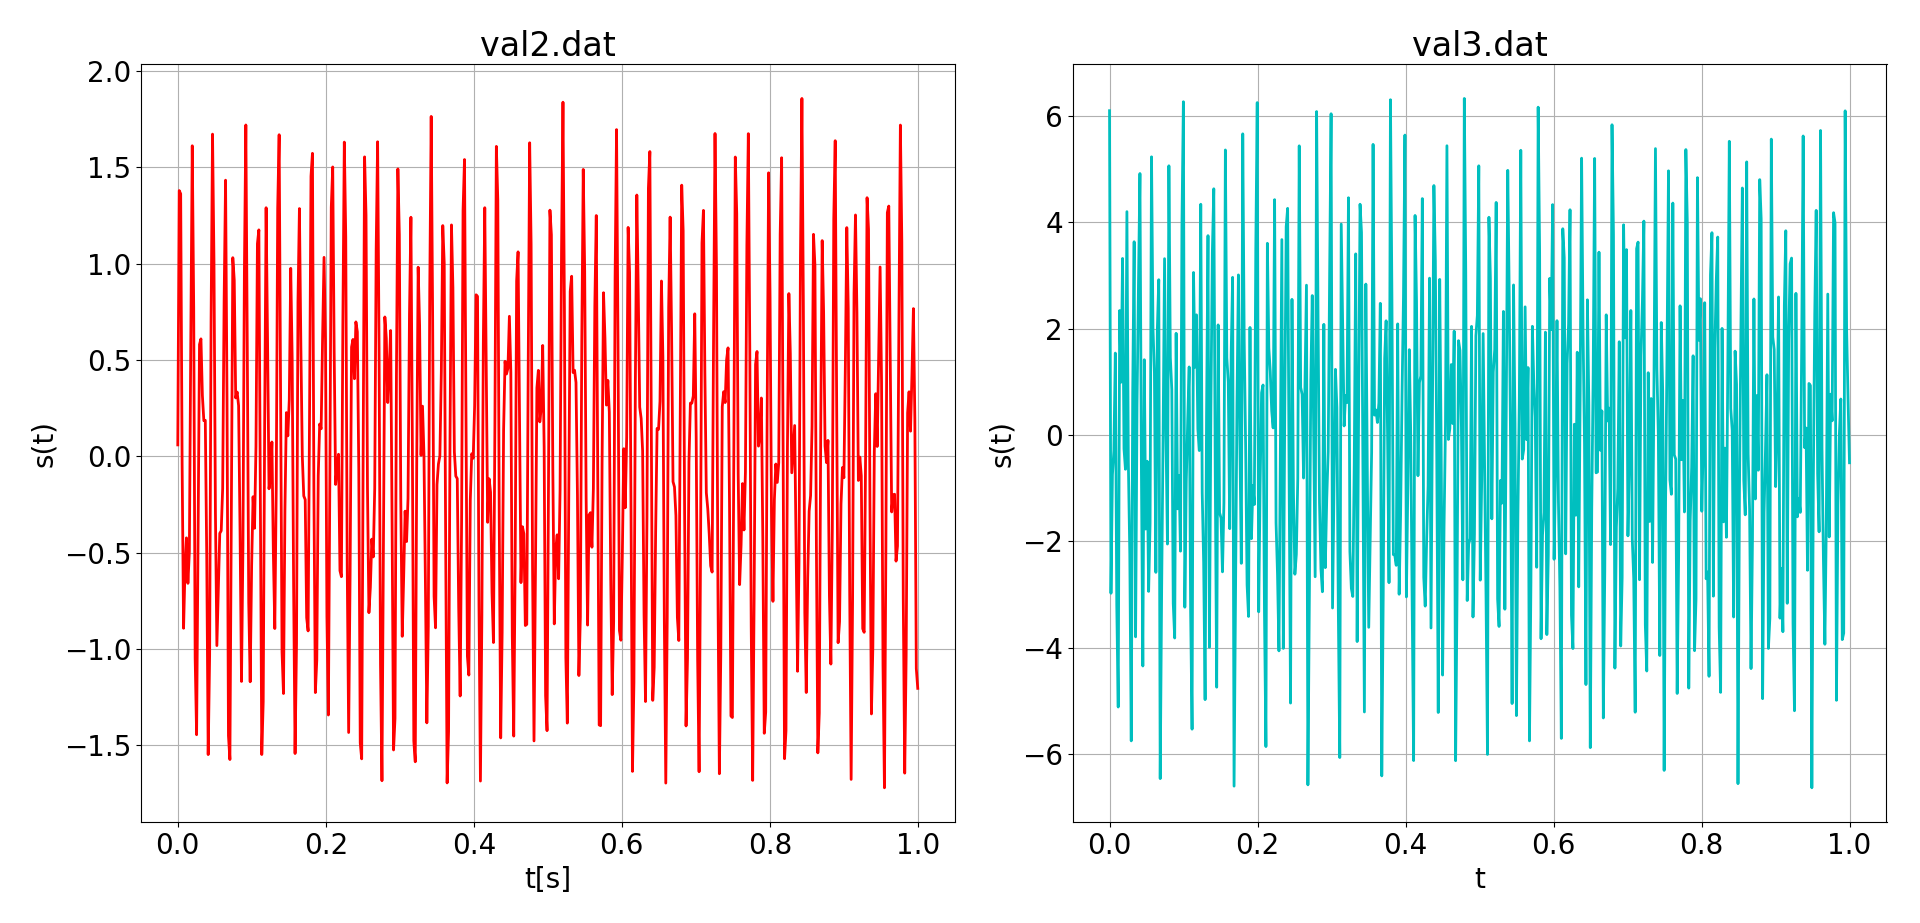
\includegraphics[width=14cm, height=5cm]{prva_prvi.png}
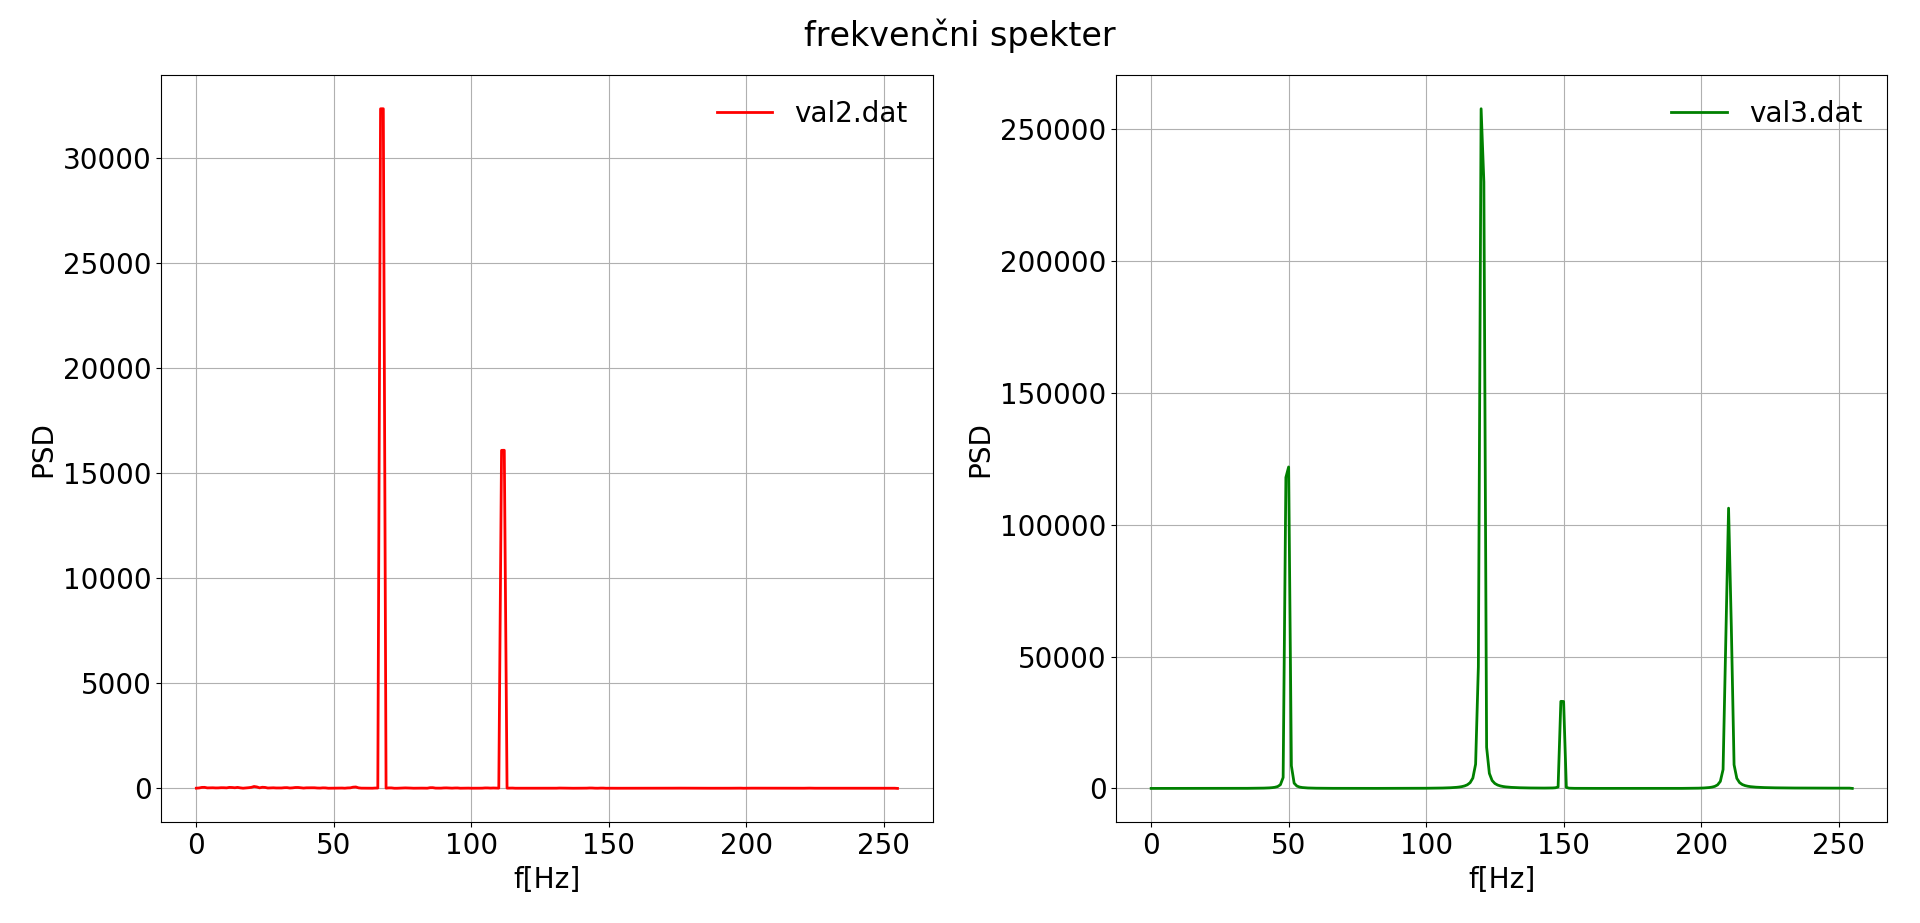
\includegraphics[width=13.5cm, height=5cm]{prva_prvi2.png}
\caption{Prikaz signalov (zgoraj) in spektralne gosotote (spodaj)}  
\end{figure}
\subsection{Vpliv izbora točk na spekter}
Poglejmo si kaj se zgodi, če vzamoe le prvih 64,128,256 točk spektra in naredimo FFT. Seveda se frekvenca samplanja ne spremeni, tako da naš spekter še vedno kaže do mejne Nyquistove frekvence. Ker bomo vzeli manjši del signala, bi morali še vedno najti vrhove, ki bodo izstopali iz spektra, vendar pa bodo zaradi tega ker je skala večja od njihove dejanske skale, raztegnjeni in nižji ker smo prejeli manj informacije, kar si lahko ogledamo na spodnjih grafih, kjer smo risali $log(PSD)$, da bomo lažje opazili razlike
\begin{figure}[H]
\centering
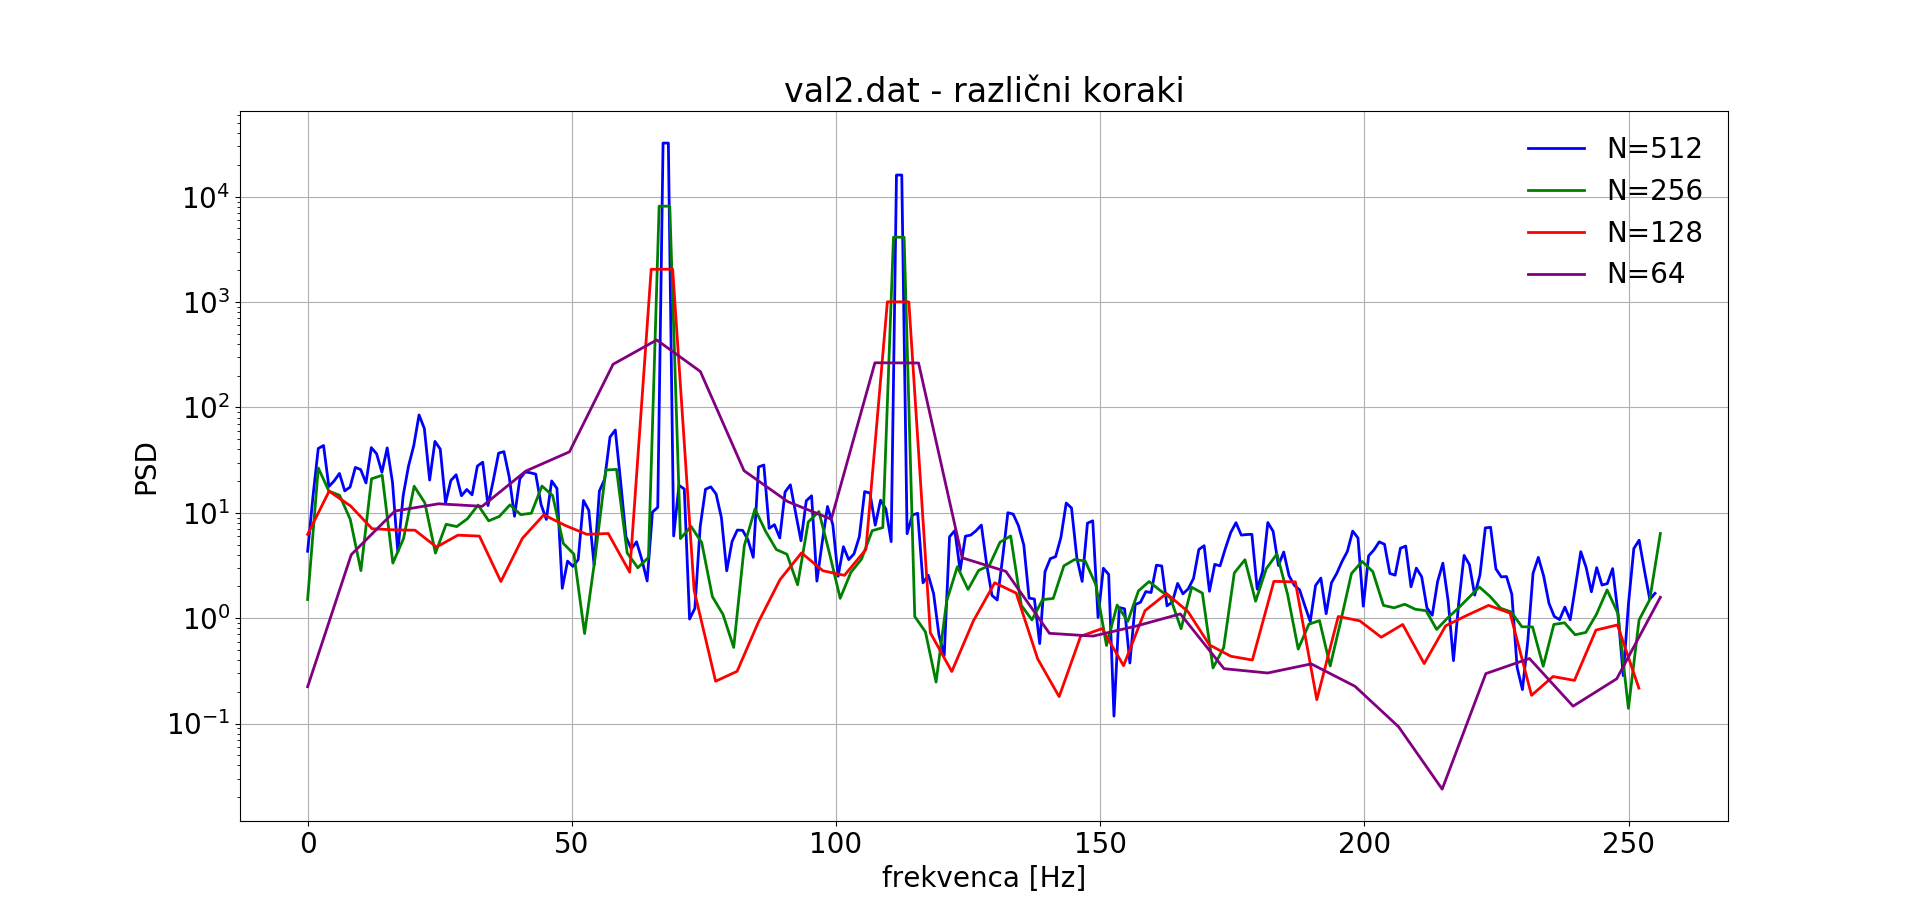
\includegraphics[width=14cm, height=6cm]{prva_drugi1.png}
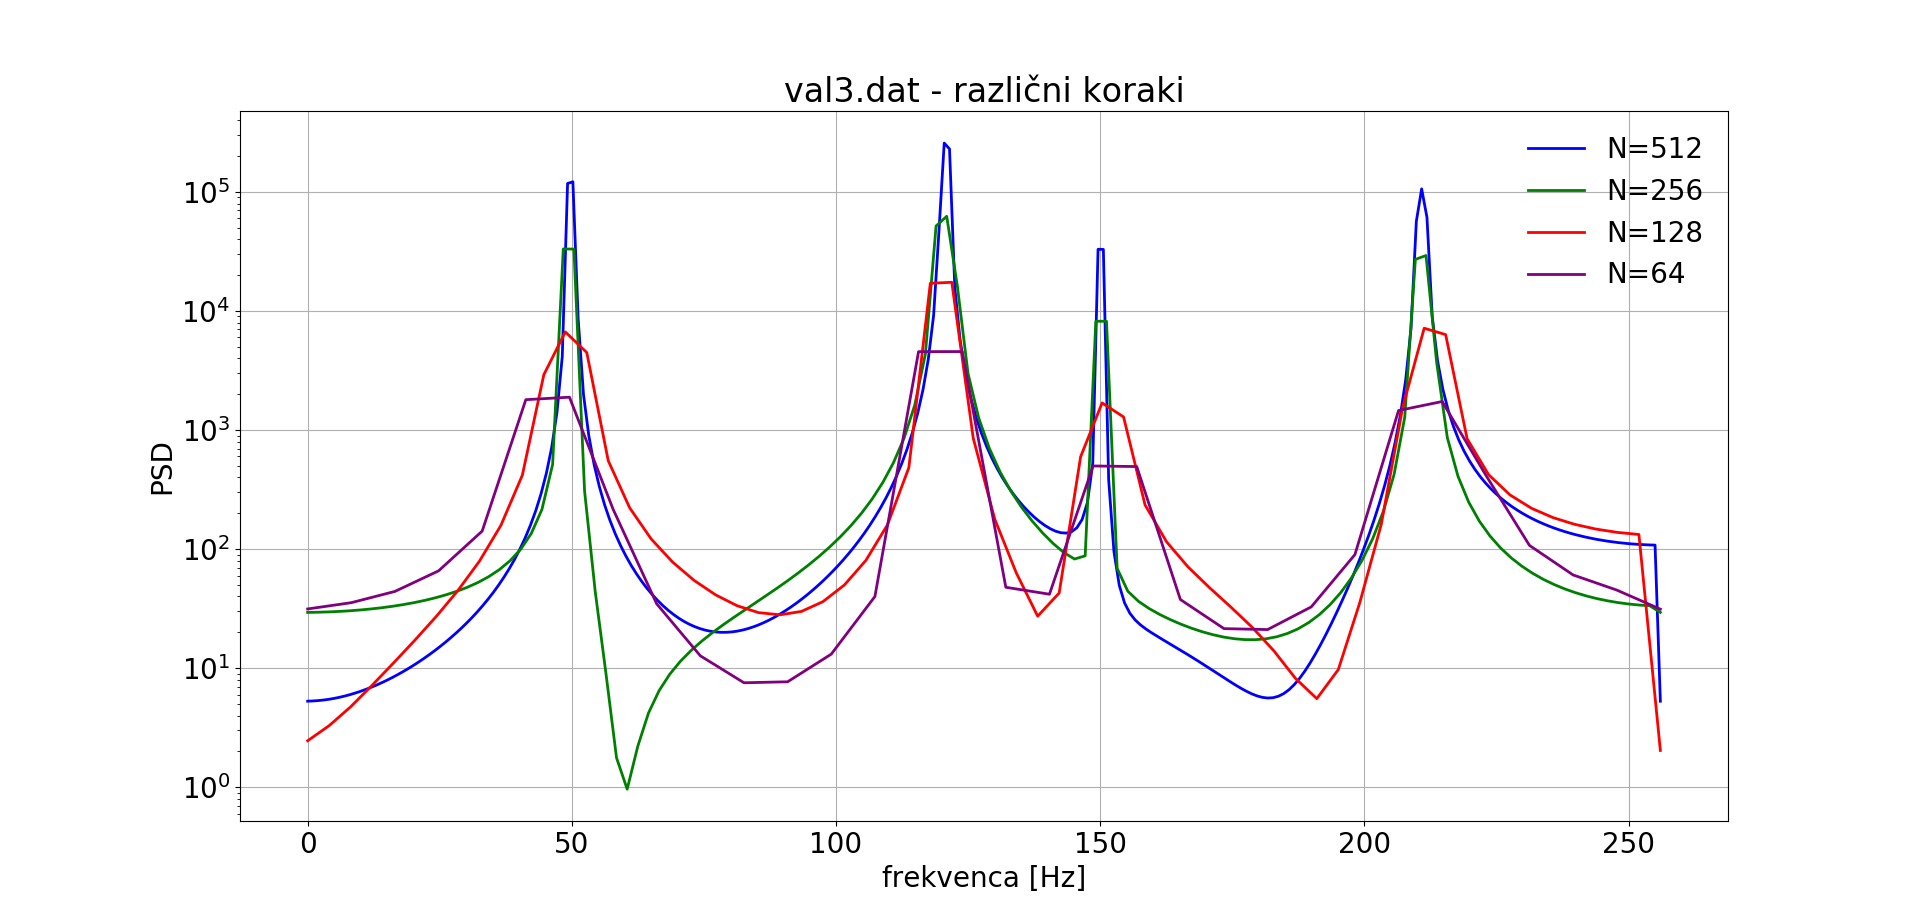
\includegraphics[width=13.5cm, height=6cm]{prva_drugi2.png}
\caption{Preiskus manjšega dela signala, nam da pričakovane rezultate. Spektralna gostota je širša in vrhovi so manjši. Zanimivo pa se mi zdi, da tudi pri 64 točkah lahko dobimo informacijo o vrhu, čeprav pa je ta sporna, saj pri spektralni analizi želimo čim večjo ločljivost frekvenc! }  
\end{figure}
\subsection{Okenske funkcije}
V nadaljevanju sem preizkusil različne okenske funkcije, s katerimi namerno deformiramo signal, da popravimo neperiodičnost našega signala. Značilnosti oken so, da so majhna na robu in čim večja na sredini, v bližini centralne transformiranke. Poznamo več vrst oken npr. \newline \textit{Welchevo okno}, definirano kot
\begin{equation}
w(n)=1 - \left(\frac{n-\frac{N-1}{2}}{\frac{N-1}{2}}\right)^2
\end{equation}
\textit{Hannovo okno}
\begin{equation}
w(n) = 0.5 \left[1 - \cos \left ( \frac{2 \pi n}{N-1} \right) \right] = \sin^2 \left ( \frac{\pi n}{N-1} \right), 
\end{equation}
 \textit{Bartlettovo okno}
\begin{equation}
w(n)=1 - \left|\frac{n-\frac{N-1}{2}}{\frac{L}{2}}\right|,
\end{equation}
kjer gre trikotno okno, za katerega vzamemo $L=N-1$. Poznamo še okno \textit{Tukey}, definirano kot
\begin{equation}
w(n) = \left\{ \begin{matrix}
\frac{1}{2} \left[1+\cos \left(\pi \left( \frac{2 n}{\alpha (N-1)}-1 \right) \right) \right]
& 0 \leqslant n < \frac{\alpha (N-1)}{2} \\ 
1 & \frac{\alpha (N-1)}{2}\leqslant n \leqslant (N-1) (1 - \frac{\alpha}{2}) \\ 
\frac{1}{2} \left[1+\cos \left(\pi \left( \frac{2 n}{\alpha (N-1)}- \frac{2}{\alpha} + 1 \right) \right) \right]
& (N-1) (1 - \frac{\alpha}{2}) < n \leqslant  (N-1) \\
\end{matrix} \right.
\end{equation}
Metode je precej preprosta, saj potrebujemo $F_k = FFT(w_n s_n)$
\begin{figure}[H]

\hspace{-2cm}
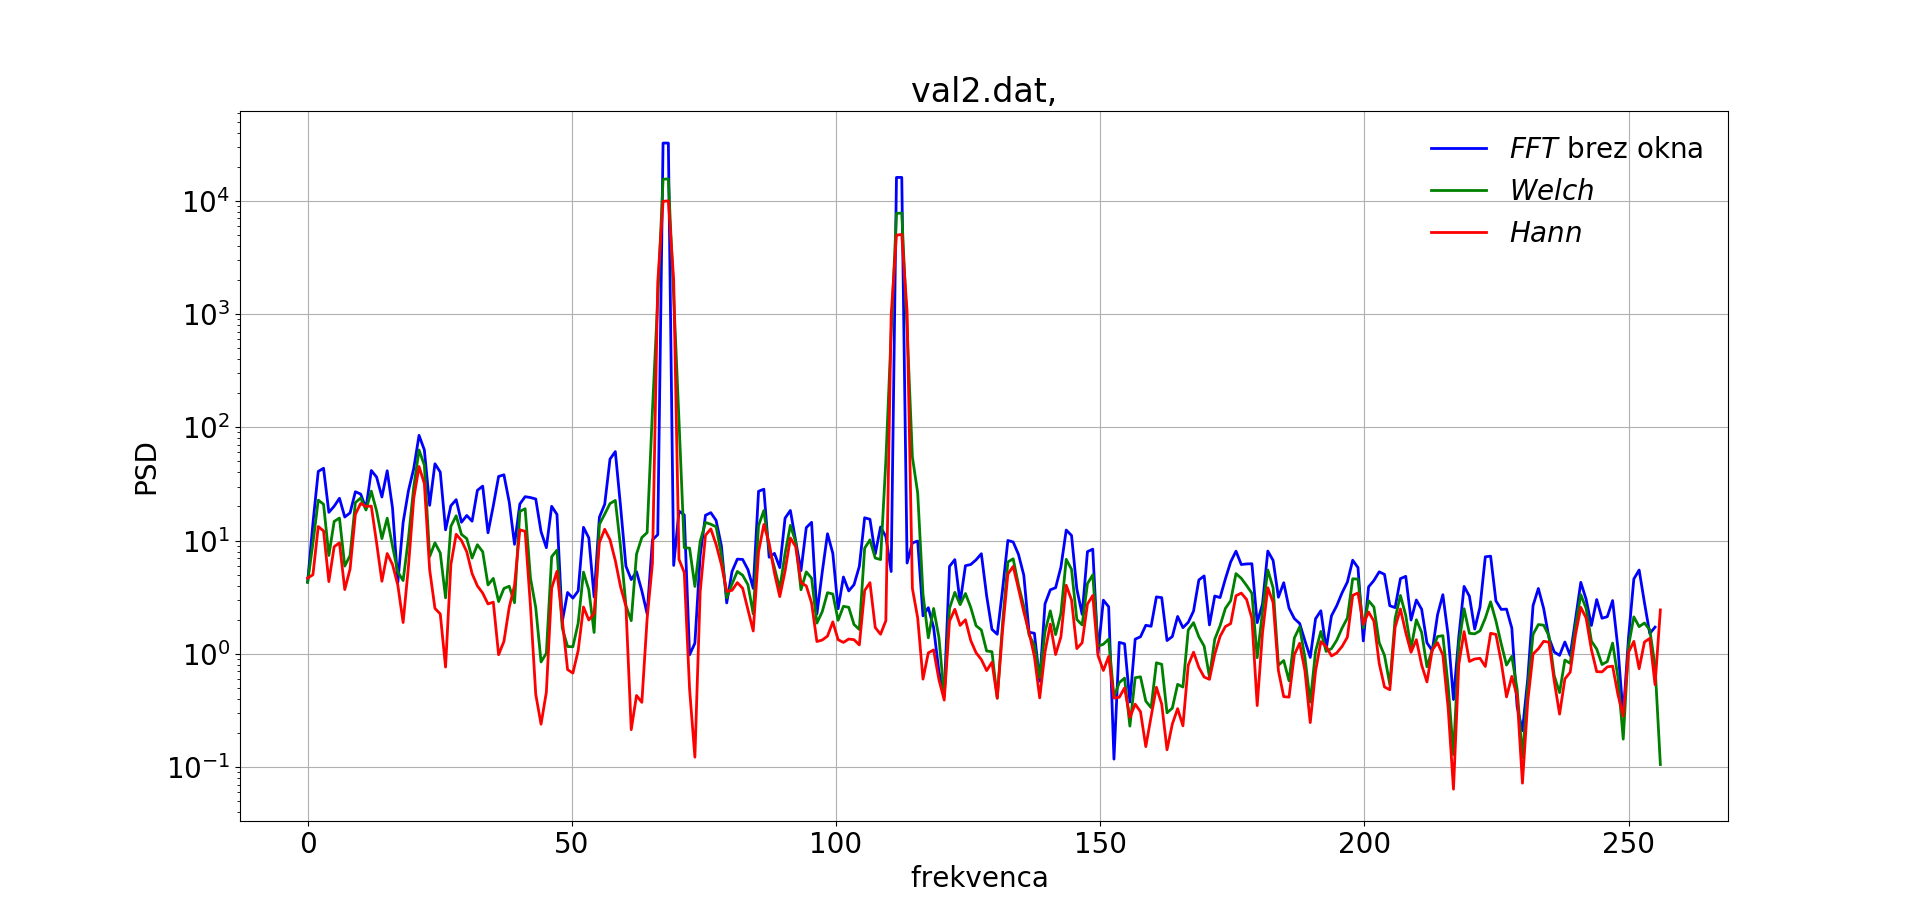
\includegraphics[width=10cm]{prva_tretji1.png}
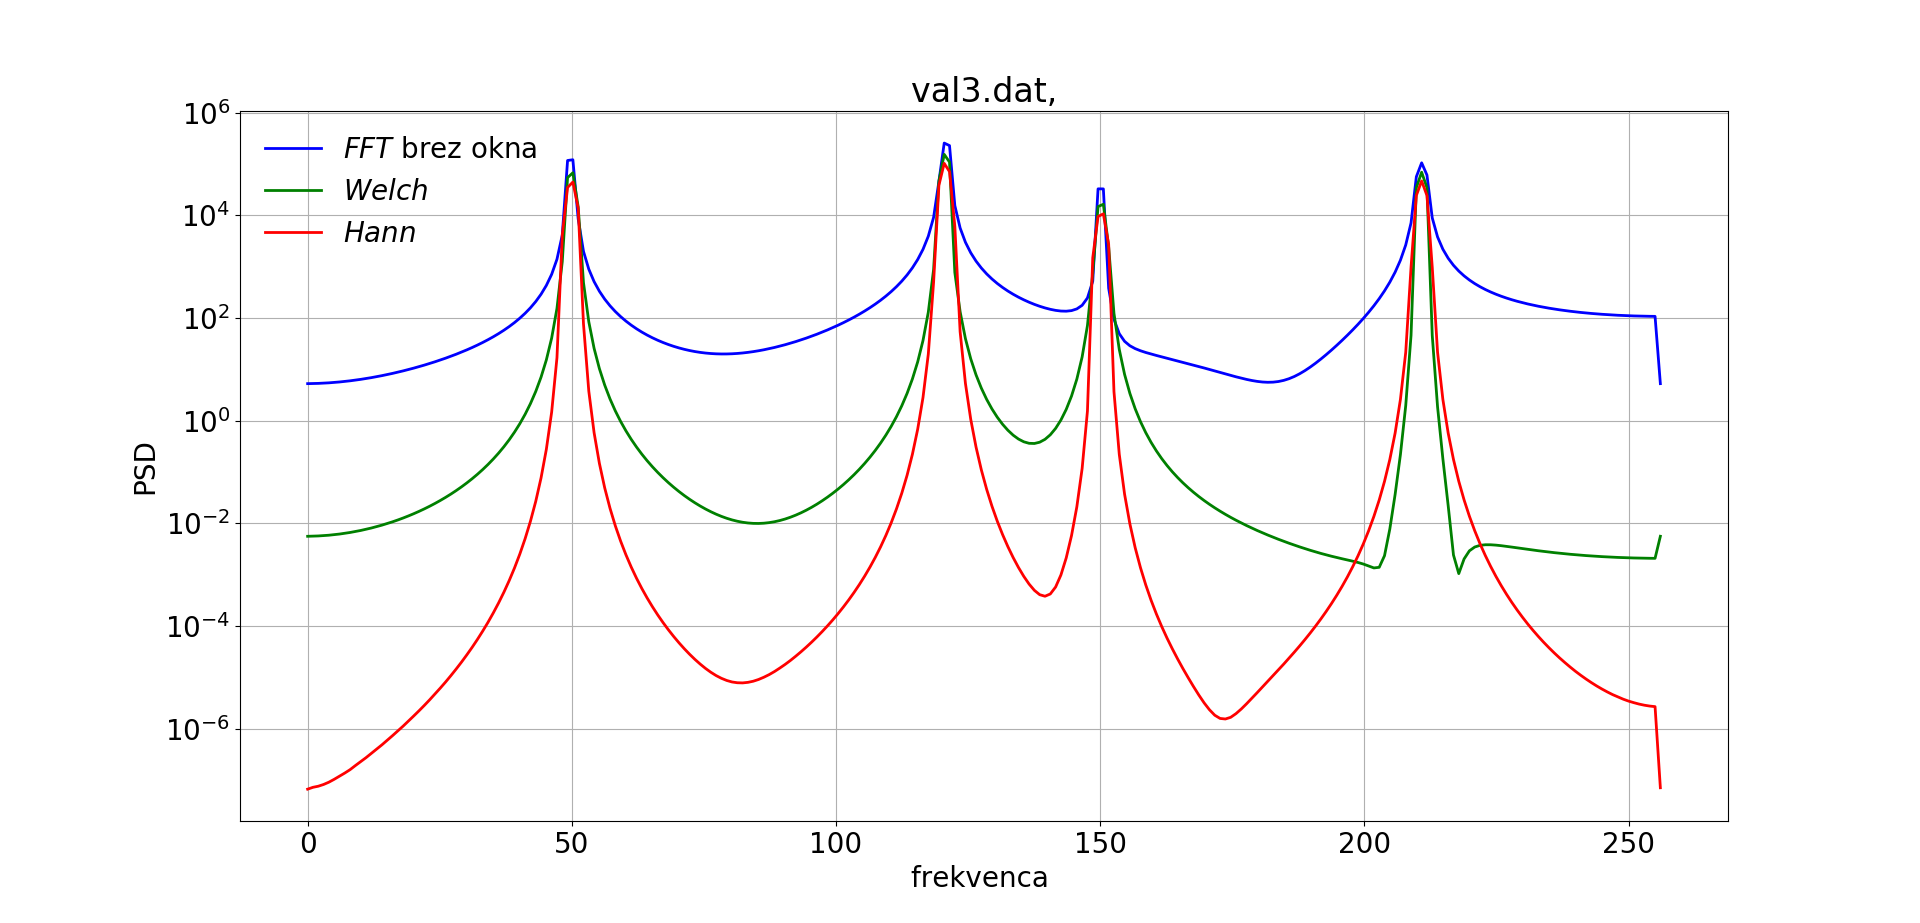
\includegraphics[width=10cm]{prva_tretja1b.png}

\caption{Prikaz okenske funkcije Welch in Hahn. Vidimo da se šum zmanjša za celo dekado, kar pomeni, da so naši vrhovi veliko bolj ostri in je šuma manj.} 
\end{figure}

\begin{figure}[H]

\hspace{-2cm}
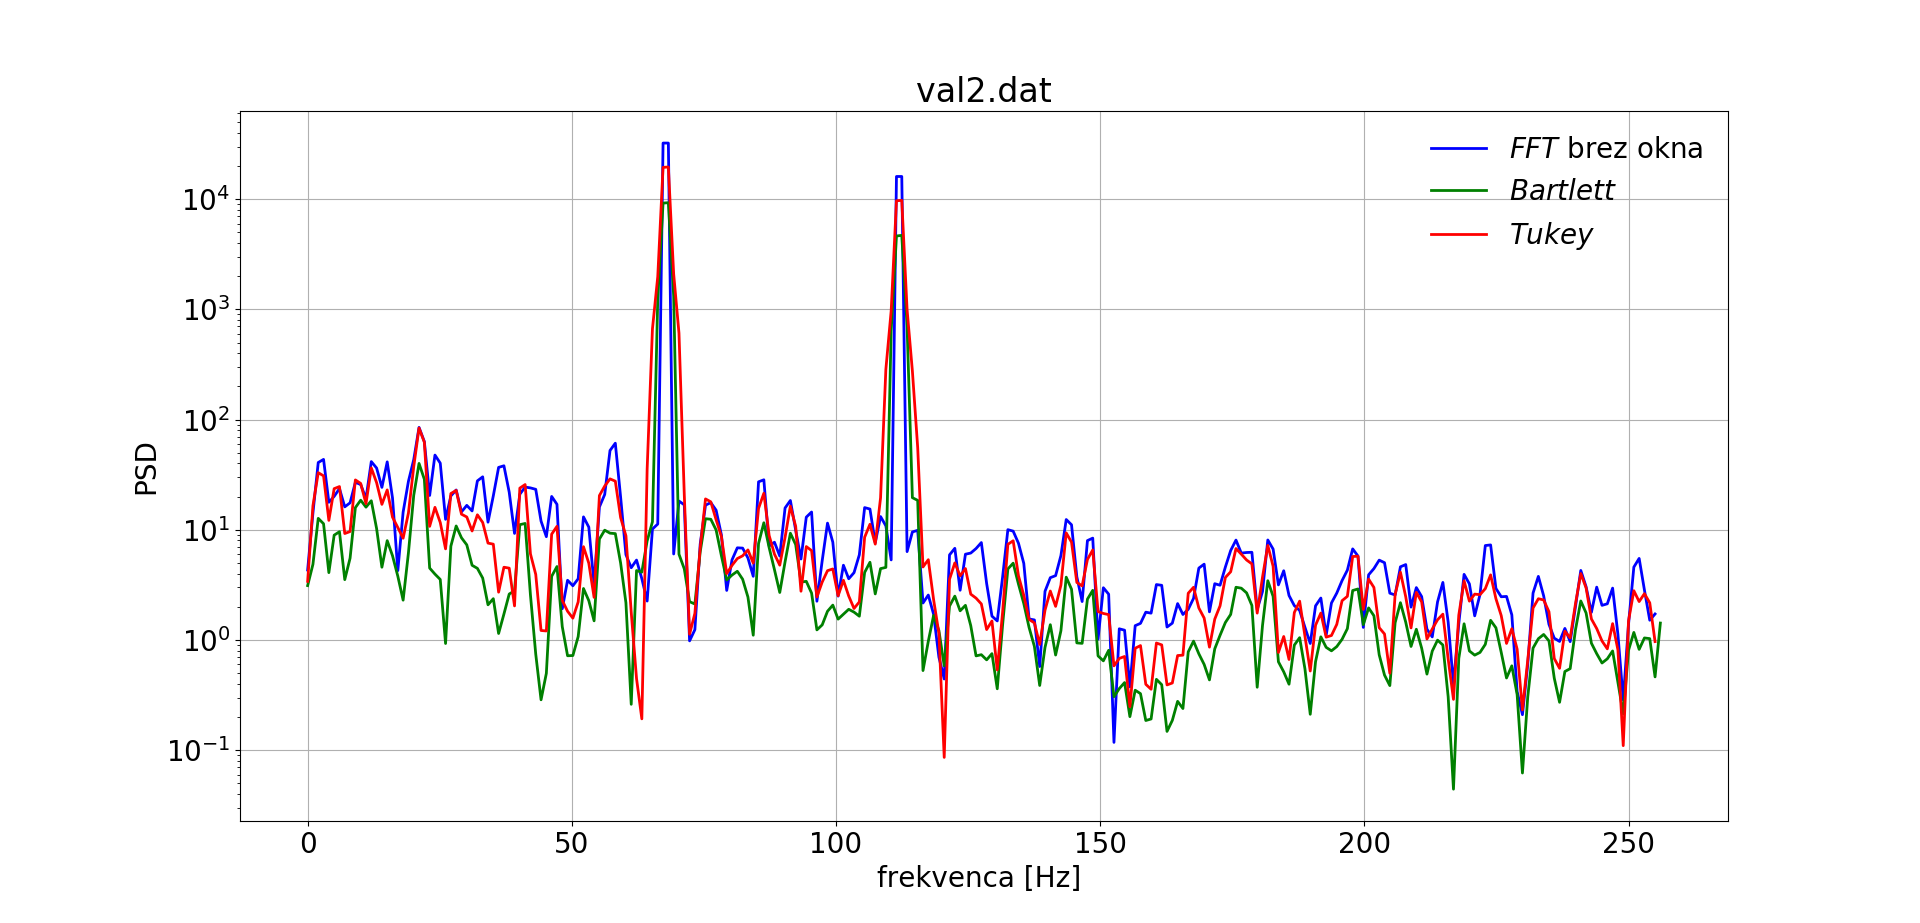
\includegraphics[width=10cm]{prva_tretji2.png}
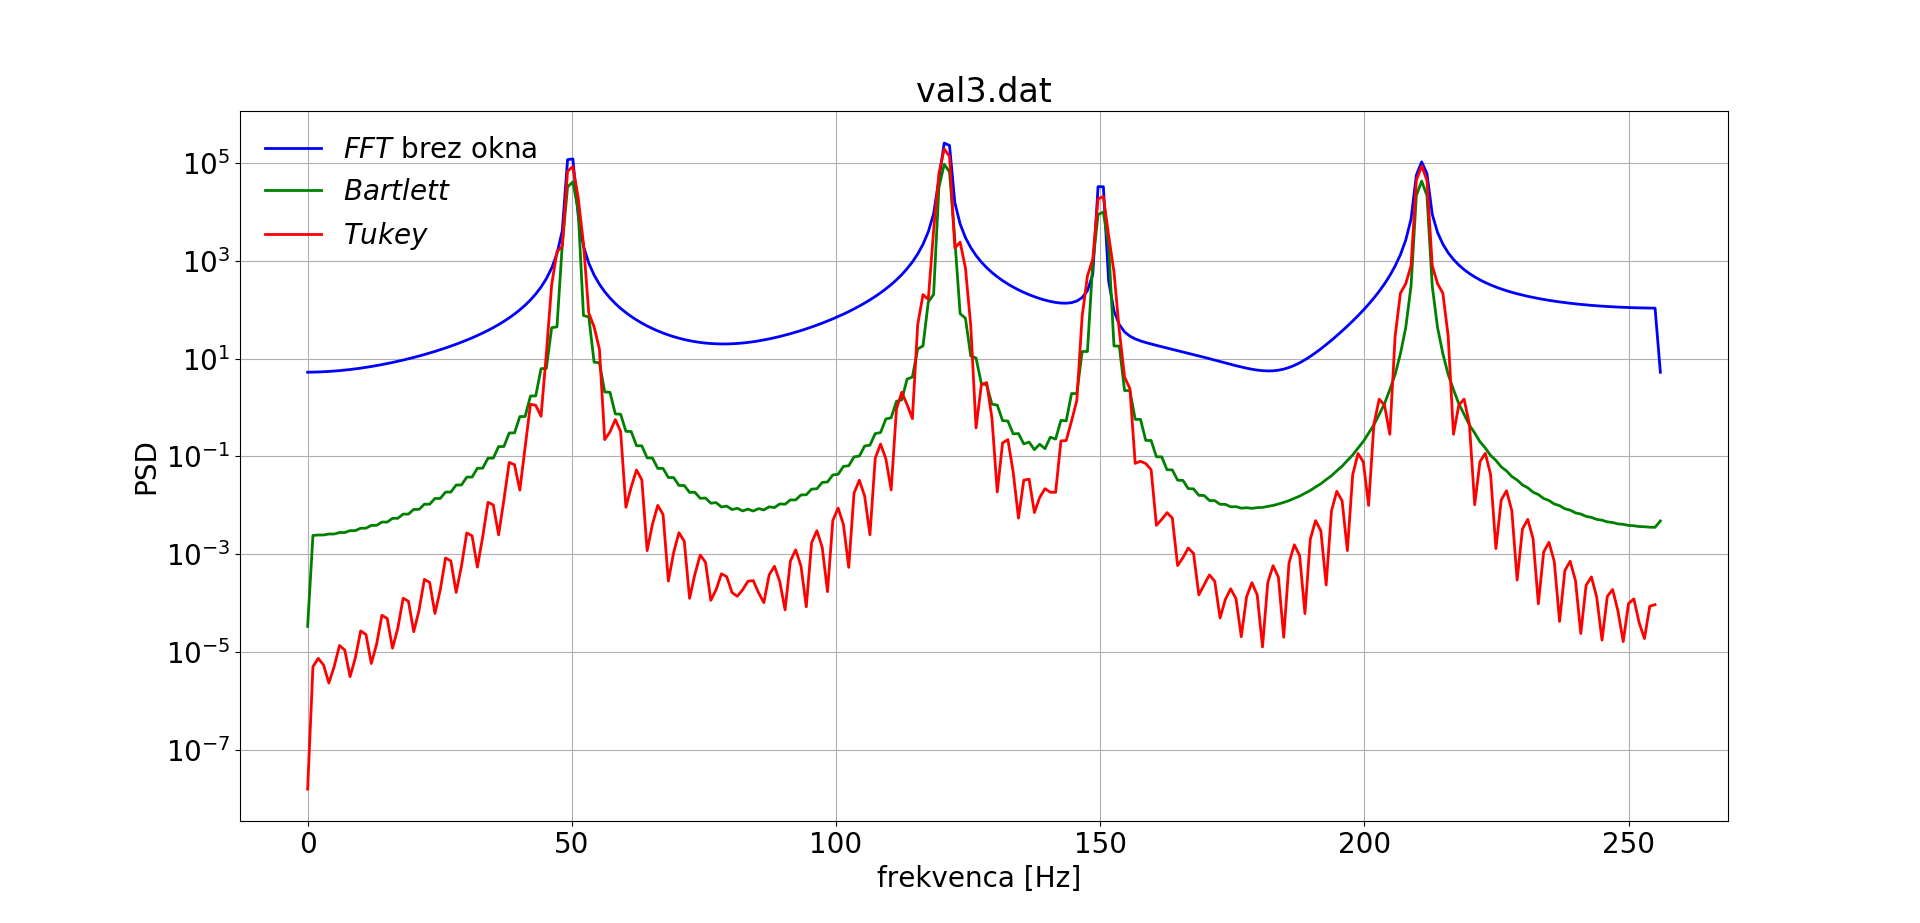
\includegraphics[width=10cm]{prva_tretji2b.png}

\caption{Prikaz okenske funkcije Bartlett, Turkey. 
Vidimo, da vsa okna popravijo naš signal in izostrijo vrhove ter zmanjšajo šum. To je seveda odvisno od našega signala, vendar pa vidimo, da na signalu $val3.dat$ na desni šum  zmanjšamo kar za 4 dekade oziroma 10 000 krat. Turkey znanimivo zaoscilira našo moč, zato se mi zdi manj priročen. Najboljše okno za naš primer je tisto ki najbolj zmanjša šum, torej $Hann$, sinusno okno in $Bartlett$ - trikotno okno, seveda pa je to odvisno od primera do primera in je verjetno treba poskusiti in opazovati katere vrhove imamo in kateri so šum.}  
\end{figure}

\section{Dekonvolucija signalov}
Recimo, da želimo meriti signal u(t). Vedno je ta signal vključen v vezje, ki ga lahko zapišemo s prenosno funkcijo r(t). Izhodni signal pa je konovlucija r(t) in u(t) ter dodatni šum zaradi vezja
\begin{equation}
c(t) = u(t) * r(t) + n(t) = s(t) + n(t)
\end{equation}
Izmerimo c(t). Zanima nas kako dobiti prvotni signal u(t). Uporabimo fourierovo transformacijo, za katero velja, da konvolucija postane množenje ustreznih transformirank
\begin{equation}
C(f) = U(f) R(f) + N(f)
\end{equation}
Če je $N(f) = 0$ lahko u(t) izračunamo kot
\begin{equation}
u(t) = FFT^{-1} [\frac{C(f)}{R(f)}]
\end{equation}
Če pa imamo šum, potem pa je ta metoda odpade in moramo najti drugačen način za približek u(t). To naredimo s pomočjo minimizacijo
\begin{equation}
\int |\widetilde{u(t)} - u(t)|^2 = \int |\widetilde{U(f)} - U(f)|^2 
\end{equation}
kjer je 
\begin{equation}
\widetilde{U(f)} = \frac{C(f)}{R(f)} \Phi(f)
\end{equation}
razpišemo in odvajamo po $\Phi$ in dobimo
\begin{equation}
\Phi(f) = \frac{|S(f)|^2}{|S(f)|^2 + |N(f)|^2}.
\end{equation}
Šuma n(t) in posledično N(f) ne poznamo eksplicitno, zato ga moramo oceniti. Tako dobimo našo oceno za signal kot
\begin{equation}
F^{-1} (\widetilde{U(f)}) = F^{-1} (\frac{C(f)}{R(f)} \Phi(f))
\end{equation}
\subsection{Signali}
Na voljo imamo 4 signale, ki naraščajo po zašumljenosti.
\begin{figure}[H]
\hspace{-2cm}
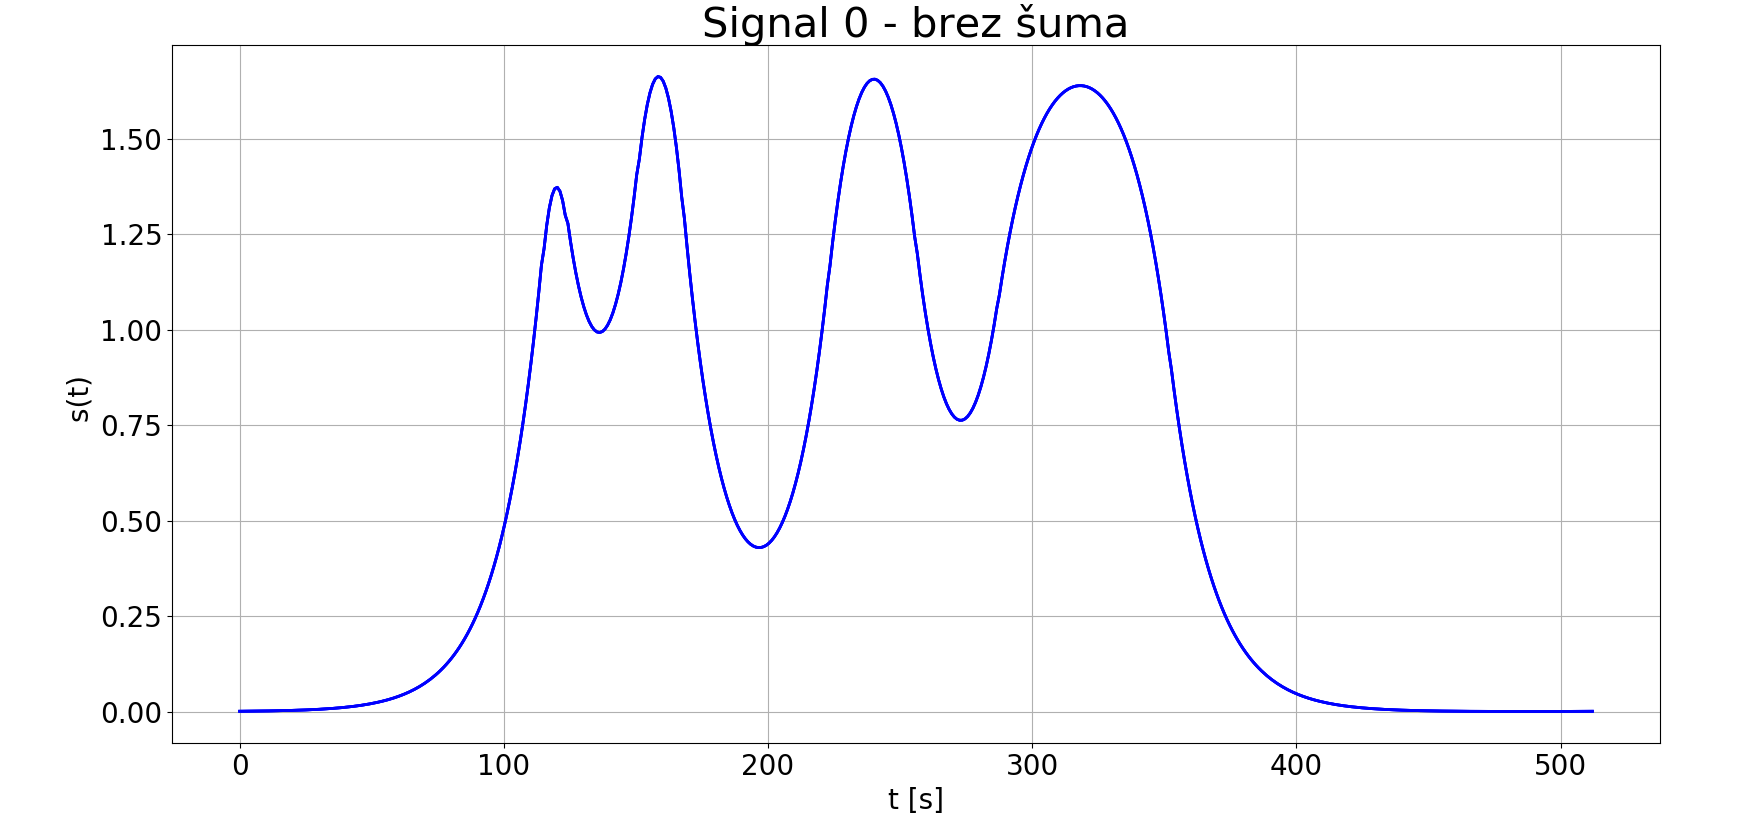
\includegraphics[width=10cm]{druga_prvi.png}
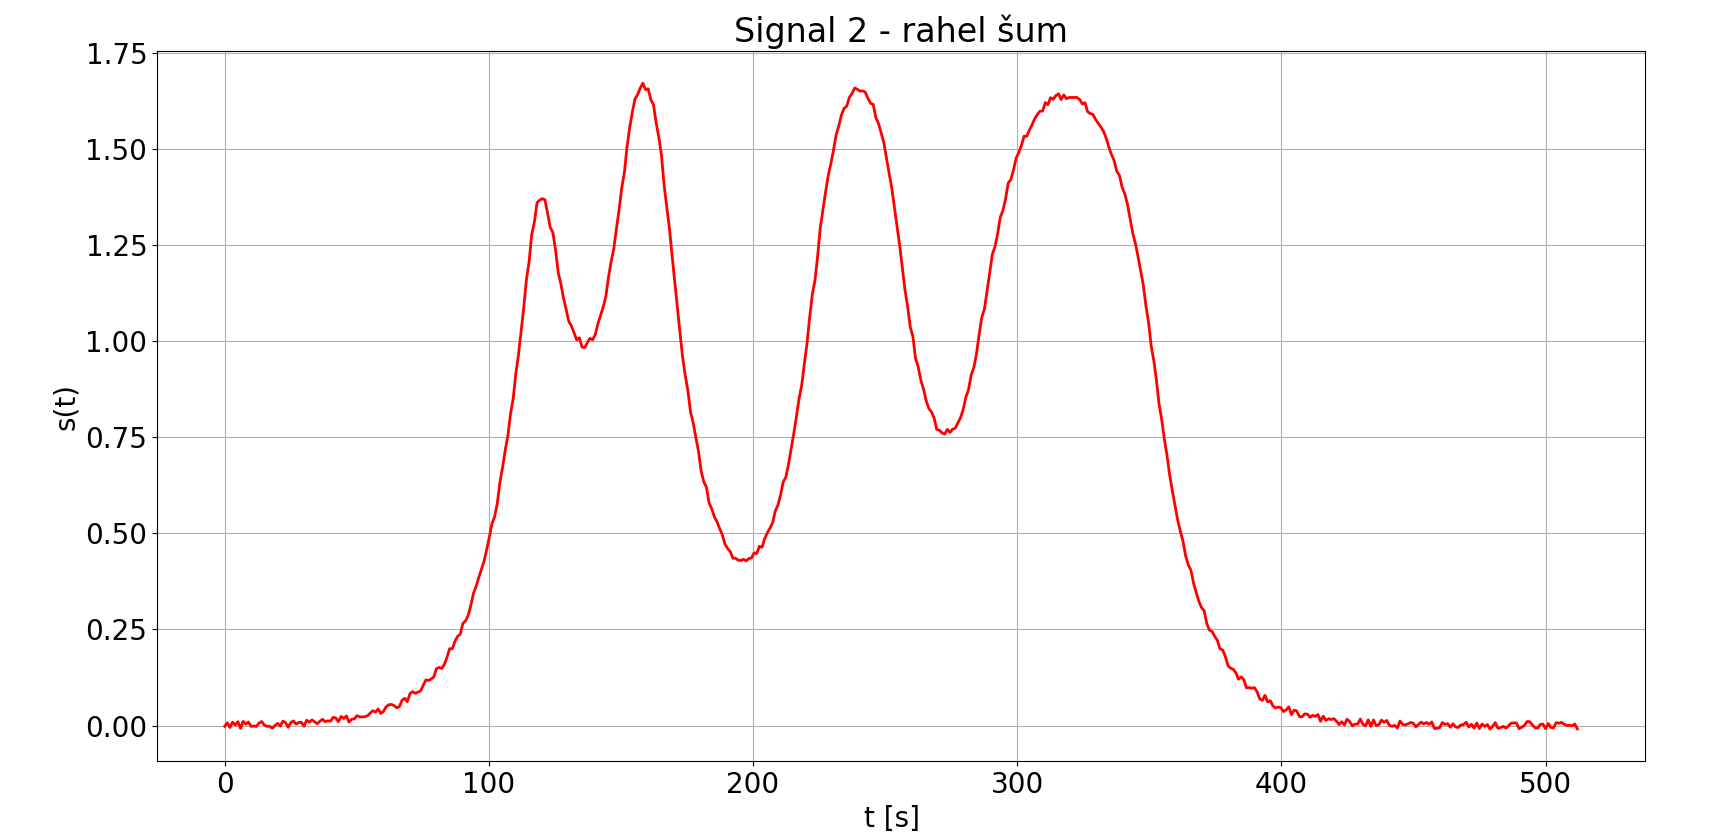
\includegraphics[width=10cm]{druga_prvi2.png}
\end{figure}
\begin{figure}[H]

\hspace{-2cm}
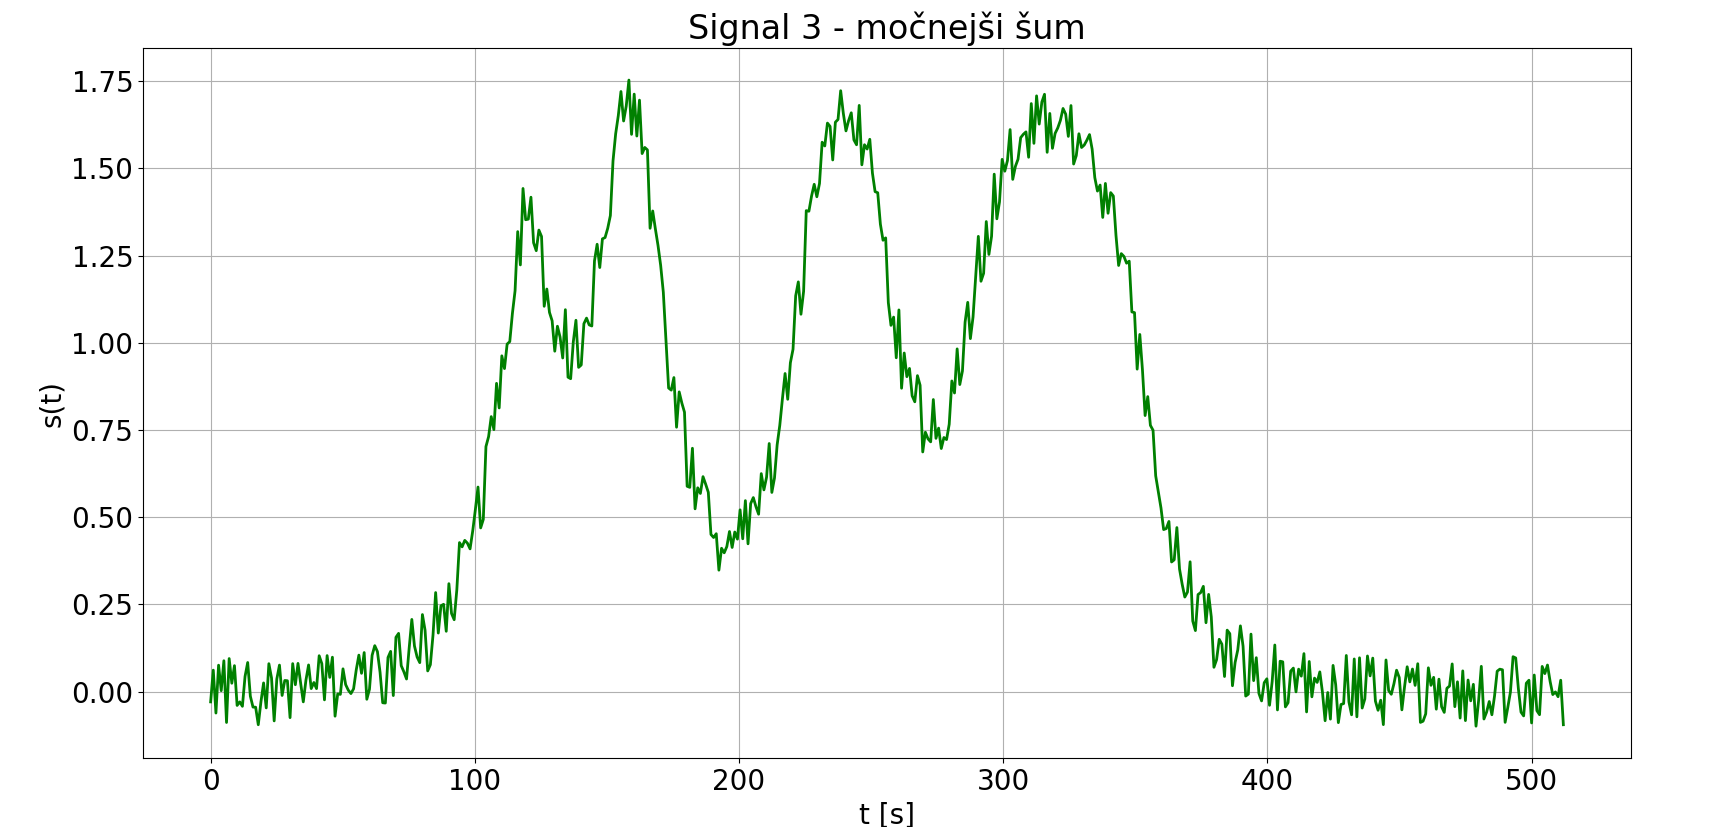
\includegraphics[width=10cm]{druga_prvi3.png}
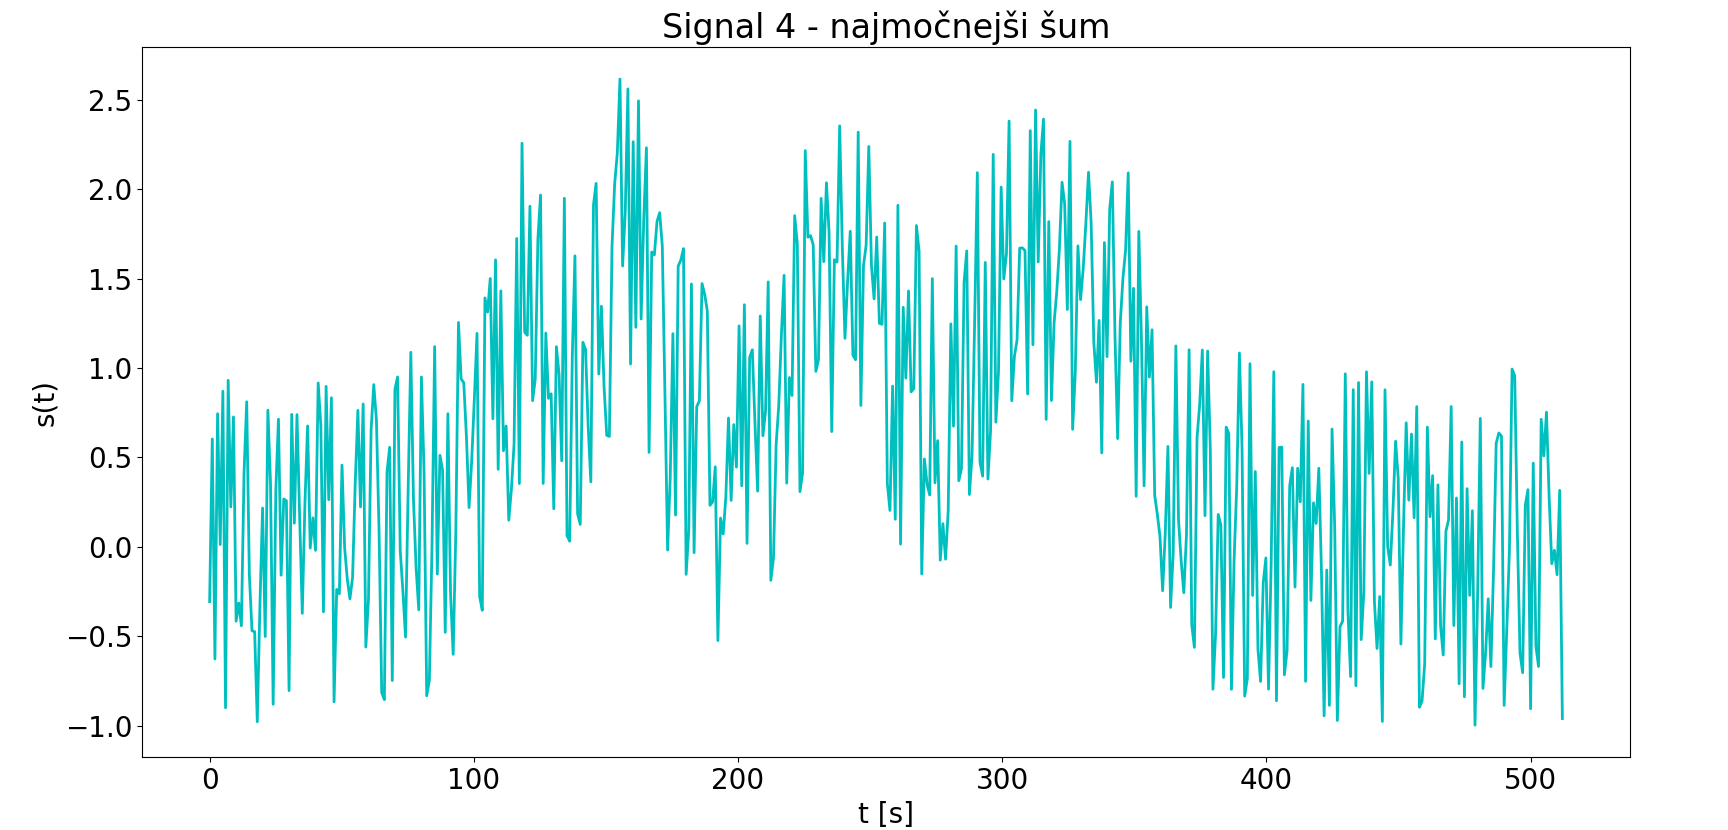
\includegraphics[width=10cm]{druga_prvi4.png}
\caption{Prikaz Signalov}
\end{figure}
\subsection{Dekonvolucija signalov}
Izmerimo, da je prenosna funkcija vezja sestavljena iz dveh eksponentnih funkcij, pri čemer je druga zrcaljena čez ordinatno os 
\begin{equation}
r(t)=\frac{1}{2 \tau} e^{\frac{-|t|}{\tau}}.
\end{equation}
Vzemimo da je $\tau = 16$ in čas samplanja $512s$ tako da je Nyquistova frekvenca $\nu_{nyquist} = 0.5 Hz$.
\begin{figure}[H]
\centering
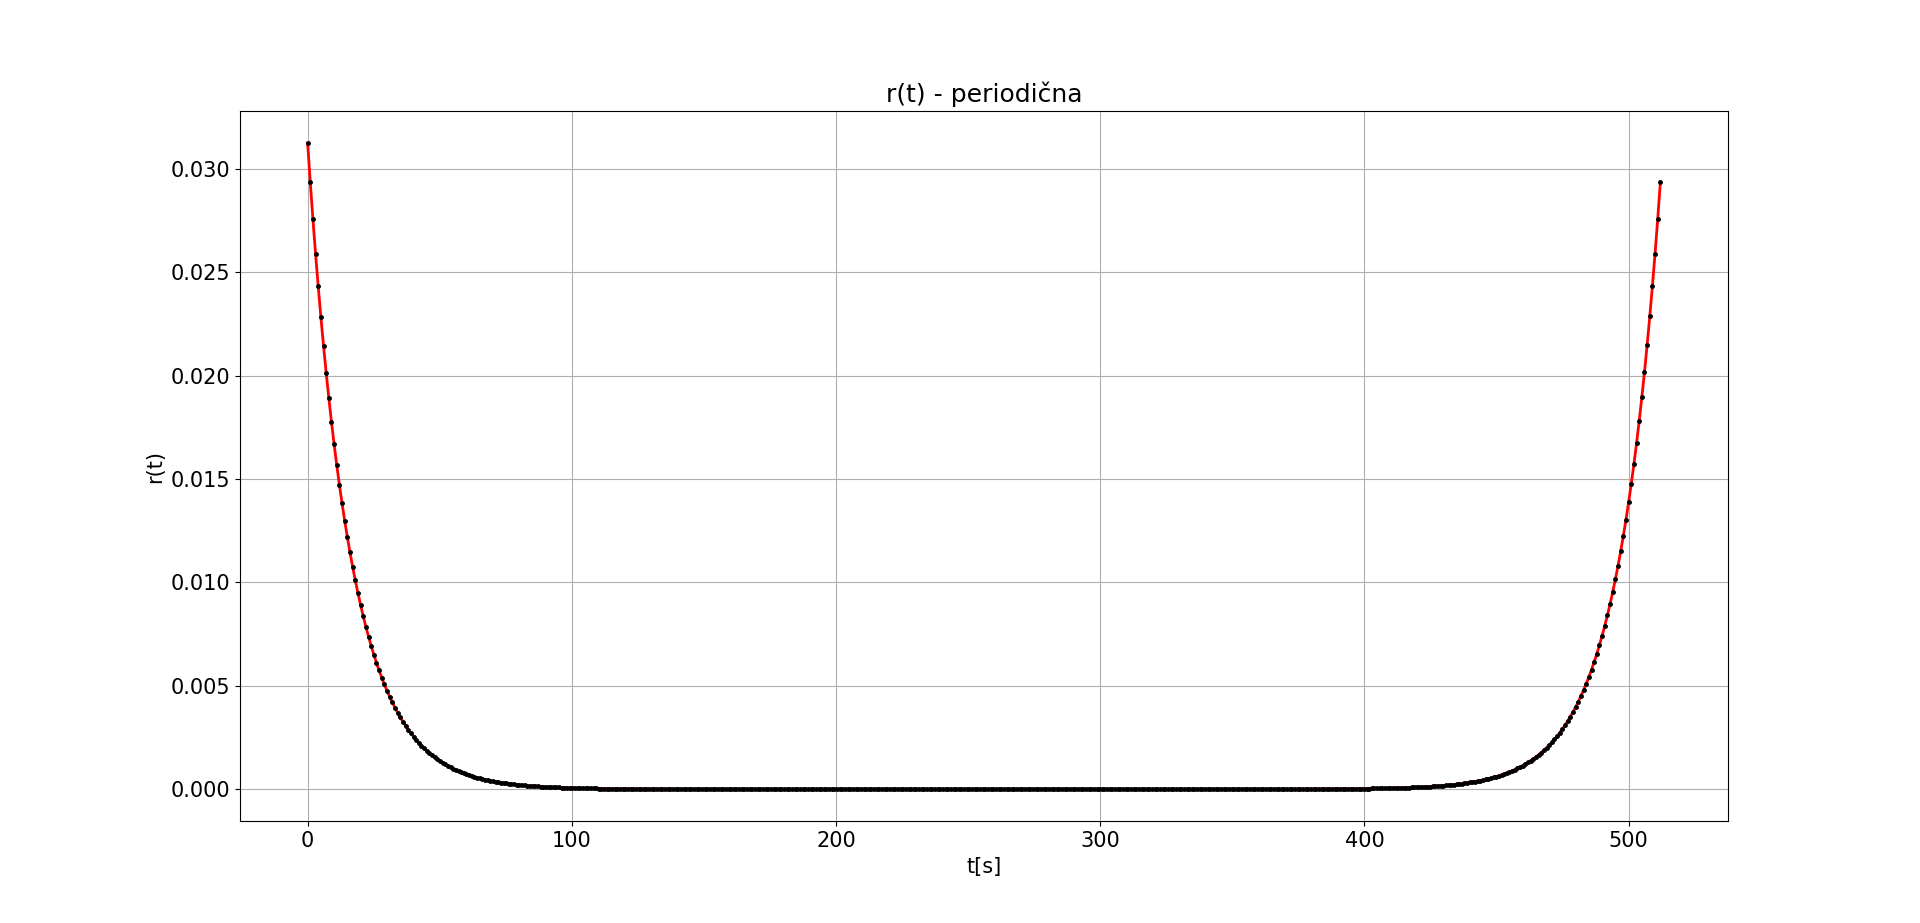
\includegraphics[width=10cm, height=6cm]{druga_drugi1.png}
\caption{Pazimo, da je r(t) periodična, tako da zadnja točka ne ponovi prve vrednosti.}  
\end{figure}
Na signalu brez šuma lahko napravimo dekonvolucijo brez Wienerjevega filtra

\begin{figure}[H]
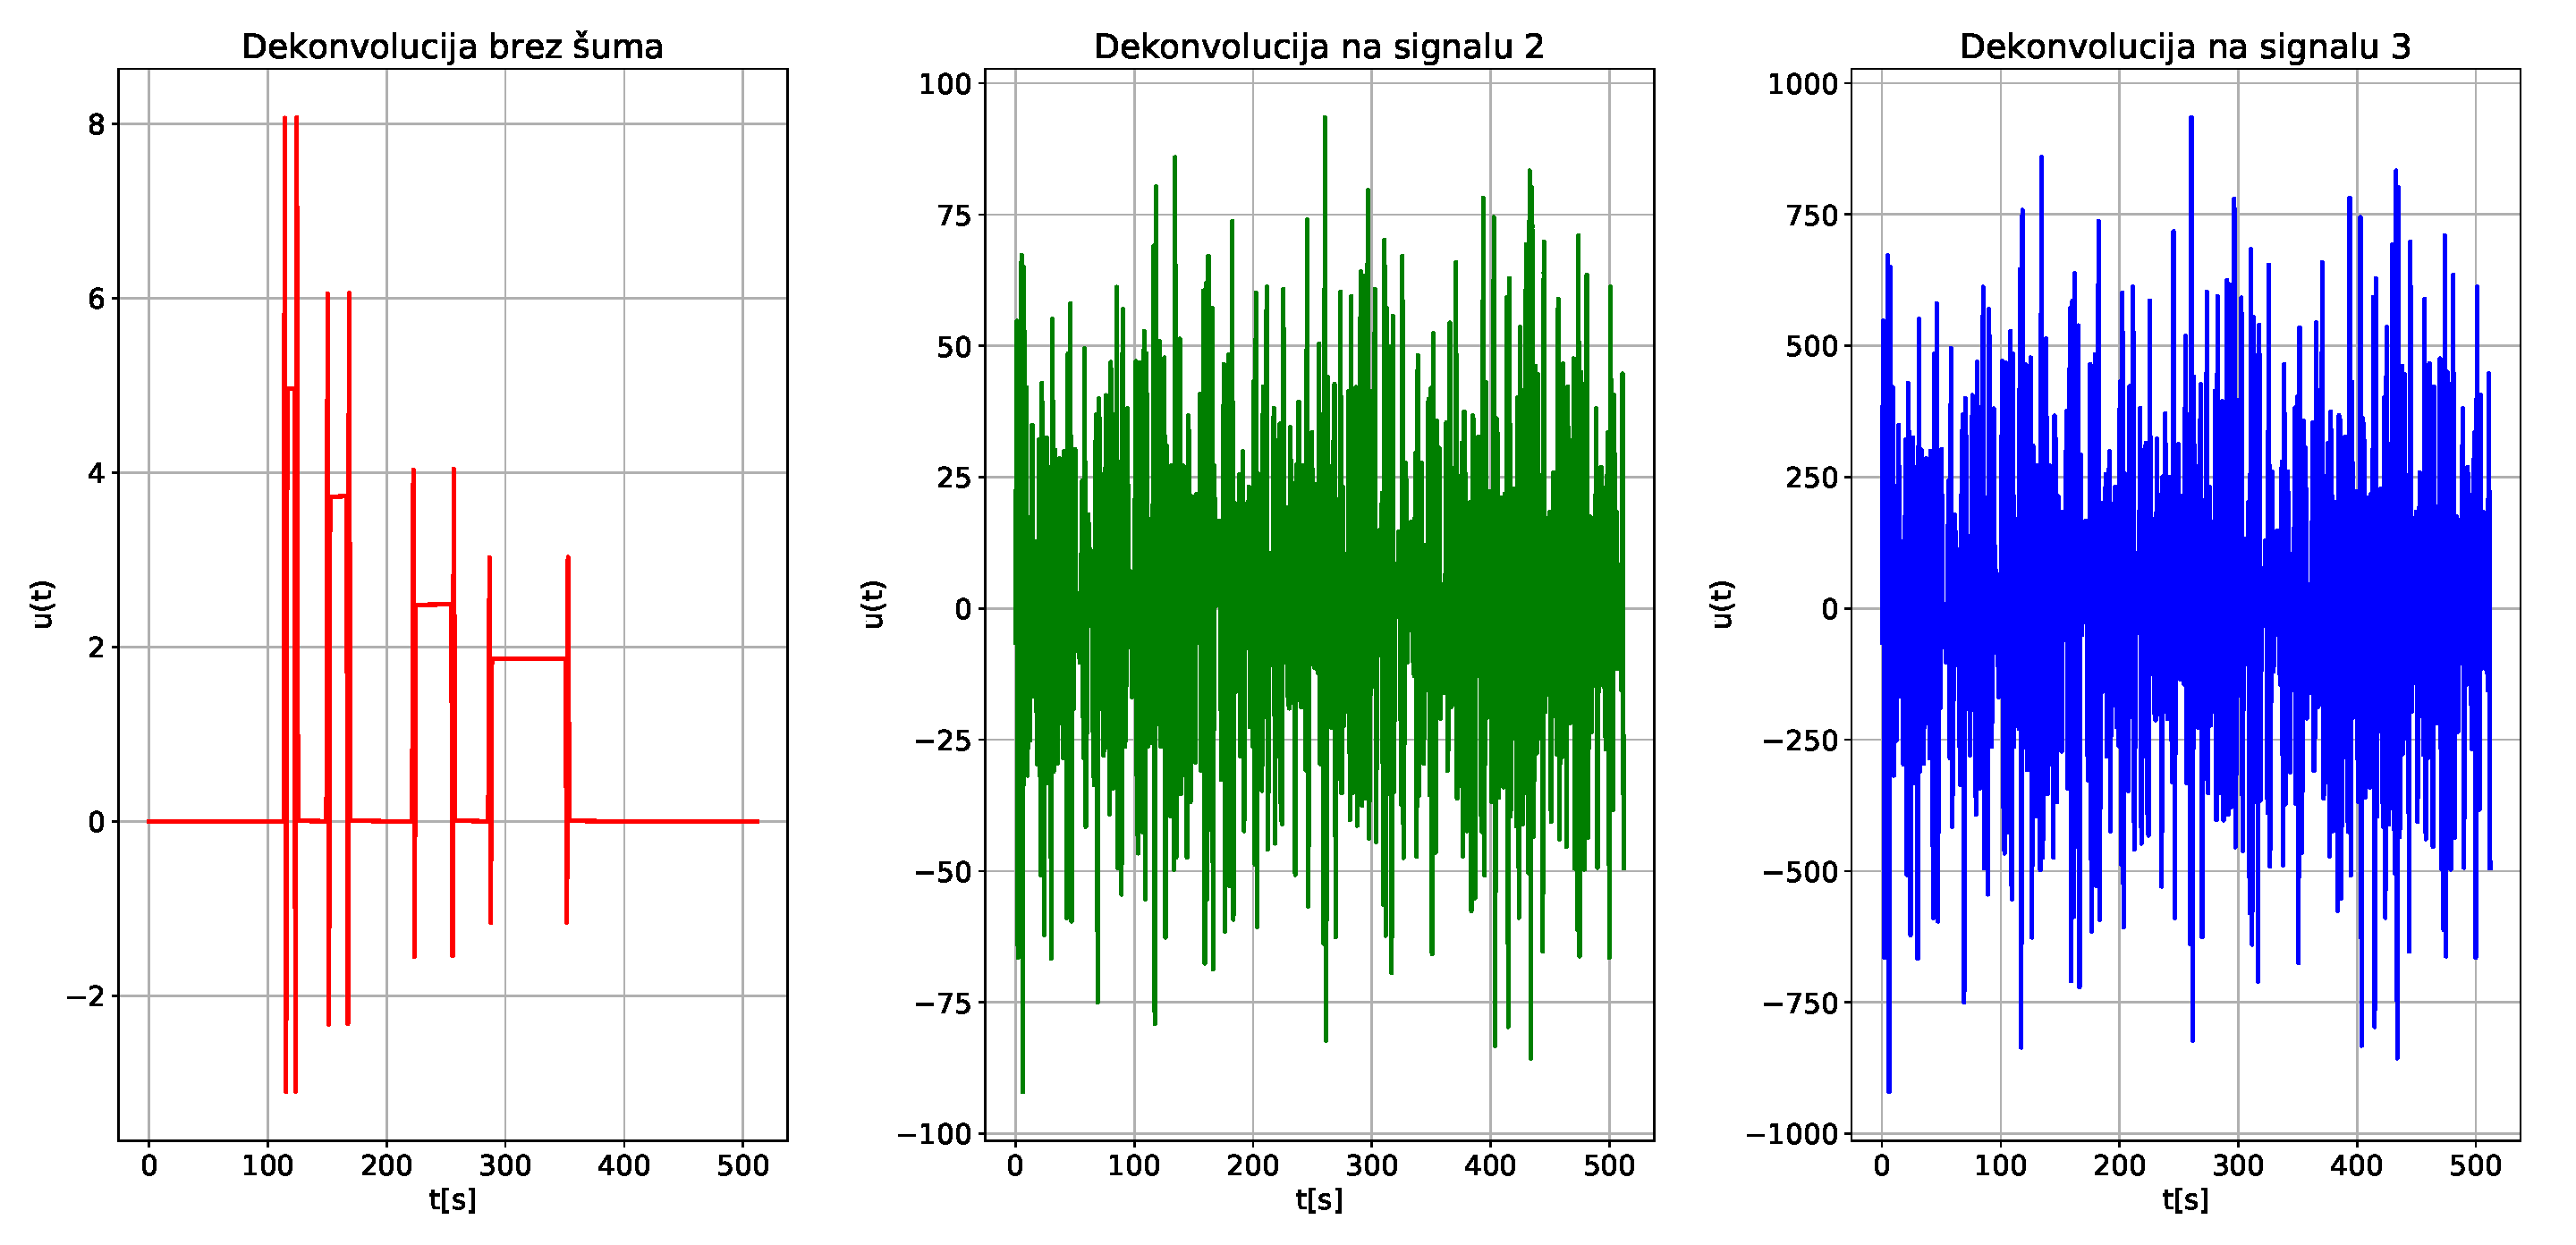
\includegraphics[width=16cm, height=6cm]{druga_drugi.pdf}
\caption{Poskus dekonvolucije brez Wienrjevega filtra, vidimo da na signalih ki so zašumljeni ne deluje več.}  
\end{figure}
Za izračun Winerjevega filtra $\Phi$ moramo oceniti $|N(f)|^2$ in $|S(f)|^2|$.  $|N(f)|^2$ ocenimo tako da narišemo spektralno moč in pogledamo kakšno je moč šuma, torej tisti del spektra, kjer se vrhovi končajo in je v povprečju konstanten. \newline\newline 
\begin{figure}[H]
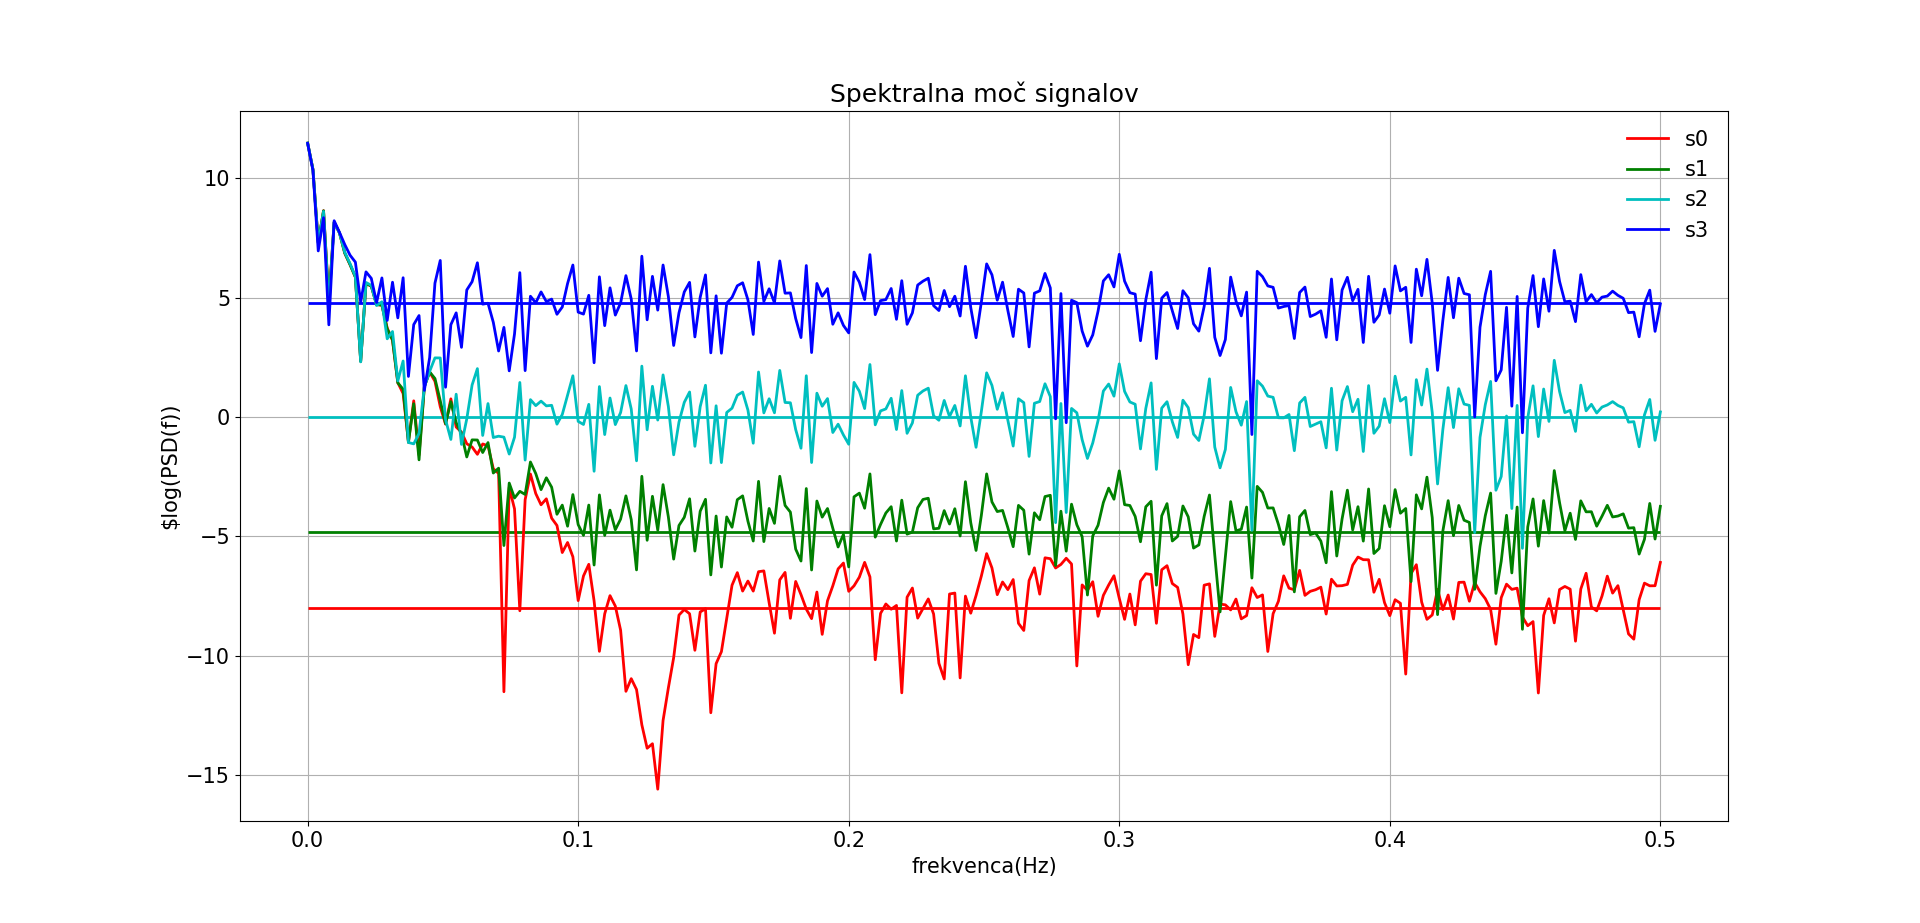
\includegraphics[width=16cm, height=6cm]{druga_drugi2.png}
\caption{Spektralna moč signalov nam da oceno za velikost šum, ki pravilno narašča z zašumljenostjo signala. Ideja je v tem, da verjetno v našem sistemu nimamo konstatne moči tako širokega spektra frekvenc in ta mora ustrezati šumu.}  
\end{figure}
Za $|S(f)|^2|$, pa imamo problem, saj je to Fourierova transformiranka signala $s(t)$ brez $n(t)$, ki pa ga mi poznamo le v začetnem delu, kjer vidimo da ima obliko premice, tako da nanj interpoliramo premico v logaritemskem prostoru oziroma $S(f) = A e^{-B f}$ v normalnem prostoru.  Paziti moramo tudi, da za fourierov obrat potrebujemo tudi negativni del spektra in tako tudi na negativni strani interpoliramo premico, ki pa jo za boljšo predstavo prezrcalimo čez ordinatno os.

\begin{figure}[H]
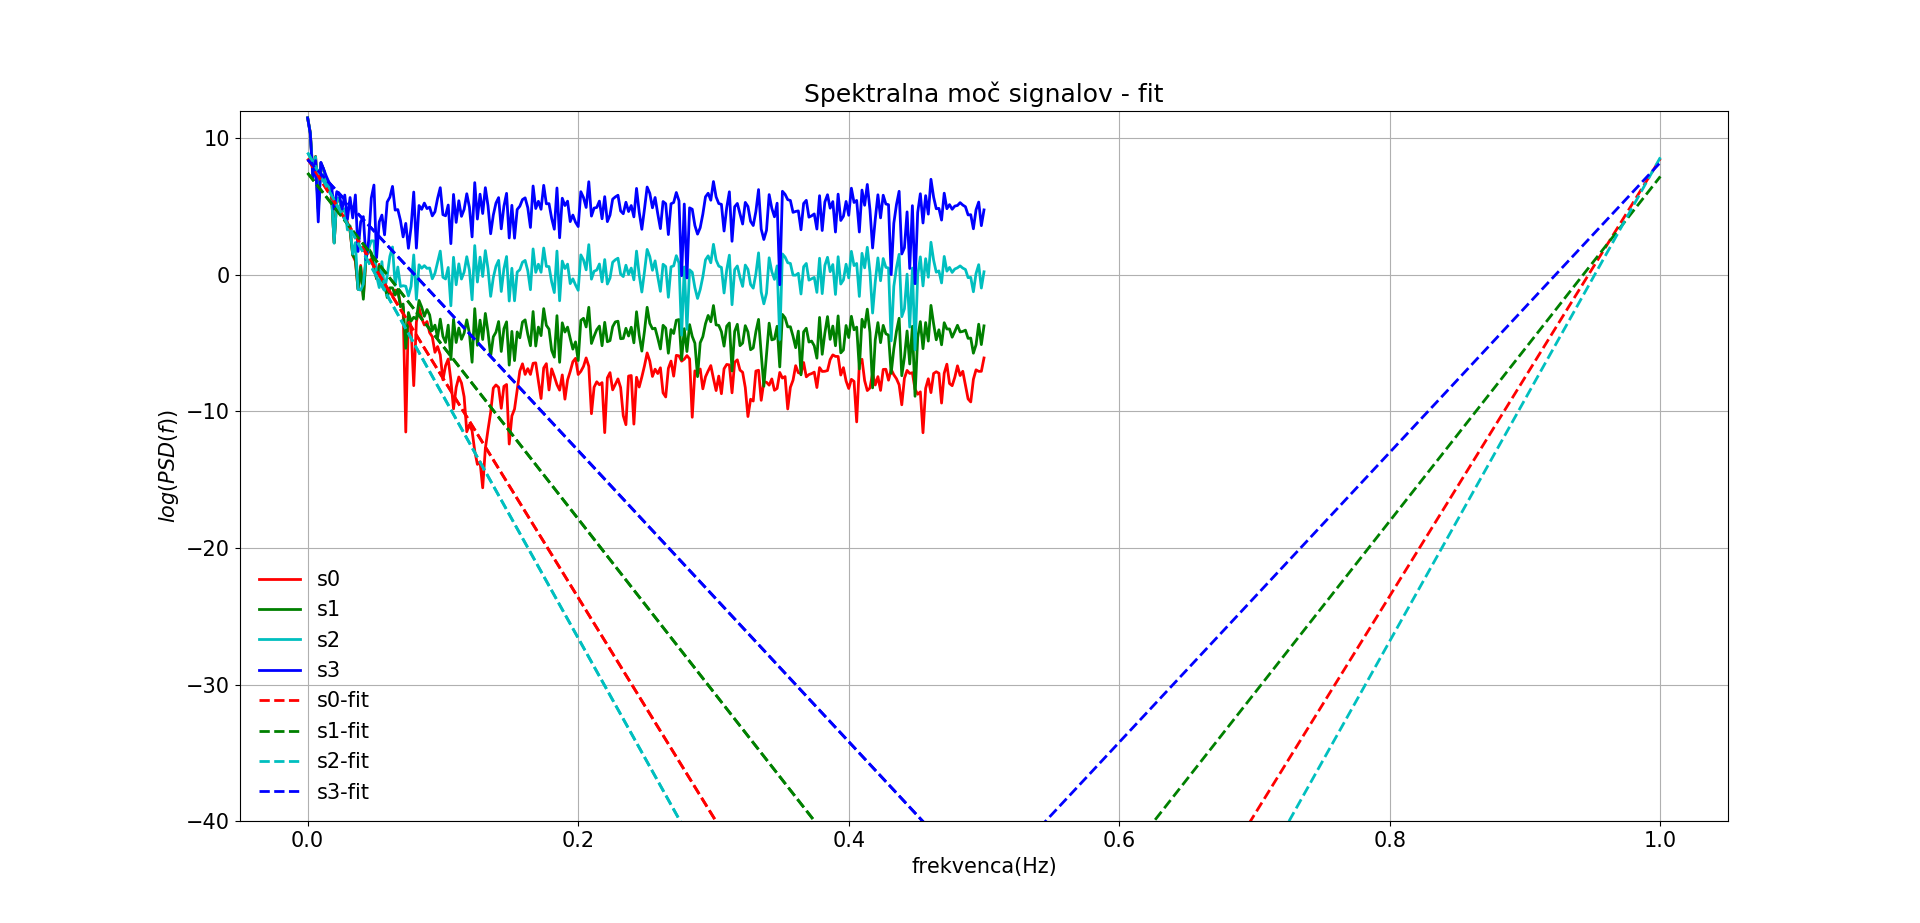
\includegraphics[width=16cm, height=6cm]{druga_drugi3fit.png}
\caption{Do neke mejne frekvence $\nu_{mejni}$, ki jo ocenimo - ko je naš spekter enak le še šumu; interpoliramo premico, ki se konča na polovici drugi del pa prezrcalimo čez ordinatno os. Paziti moramo, da zadnja točka prezrcaljene premice ni enaka začetni, da ohranimo periodičnost. Vidimo tudi da je najbolj zašumljen signal najmanj strm.}  
\end{figure}
Sedaj poznamo $|S(f)|^2|$ in $|N(f)|^2|$, ki ju moramo še pretvoriti iz logaritemske skale s pomočjo inverzne funkcije in nato lahko izračunamo $\Phi(f)$, in poskusimo s dekonvolucijo s pomočjo Wienerjevega filtra.

\begin{figure}[H]
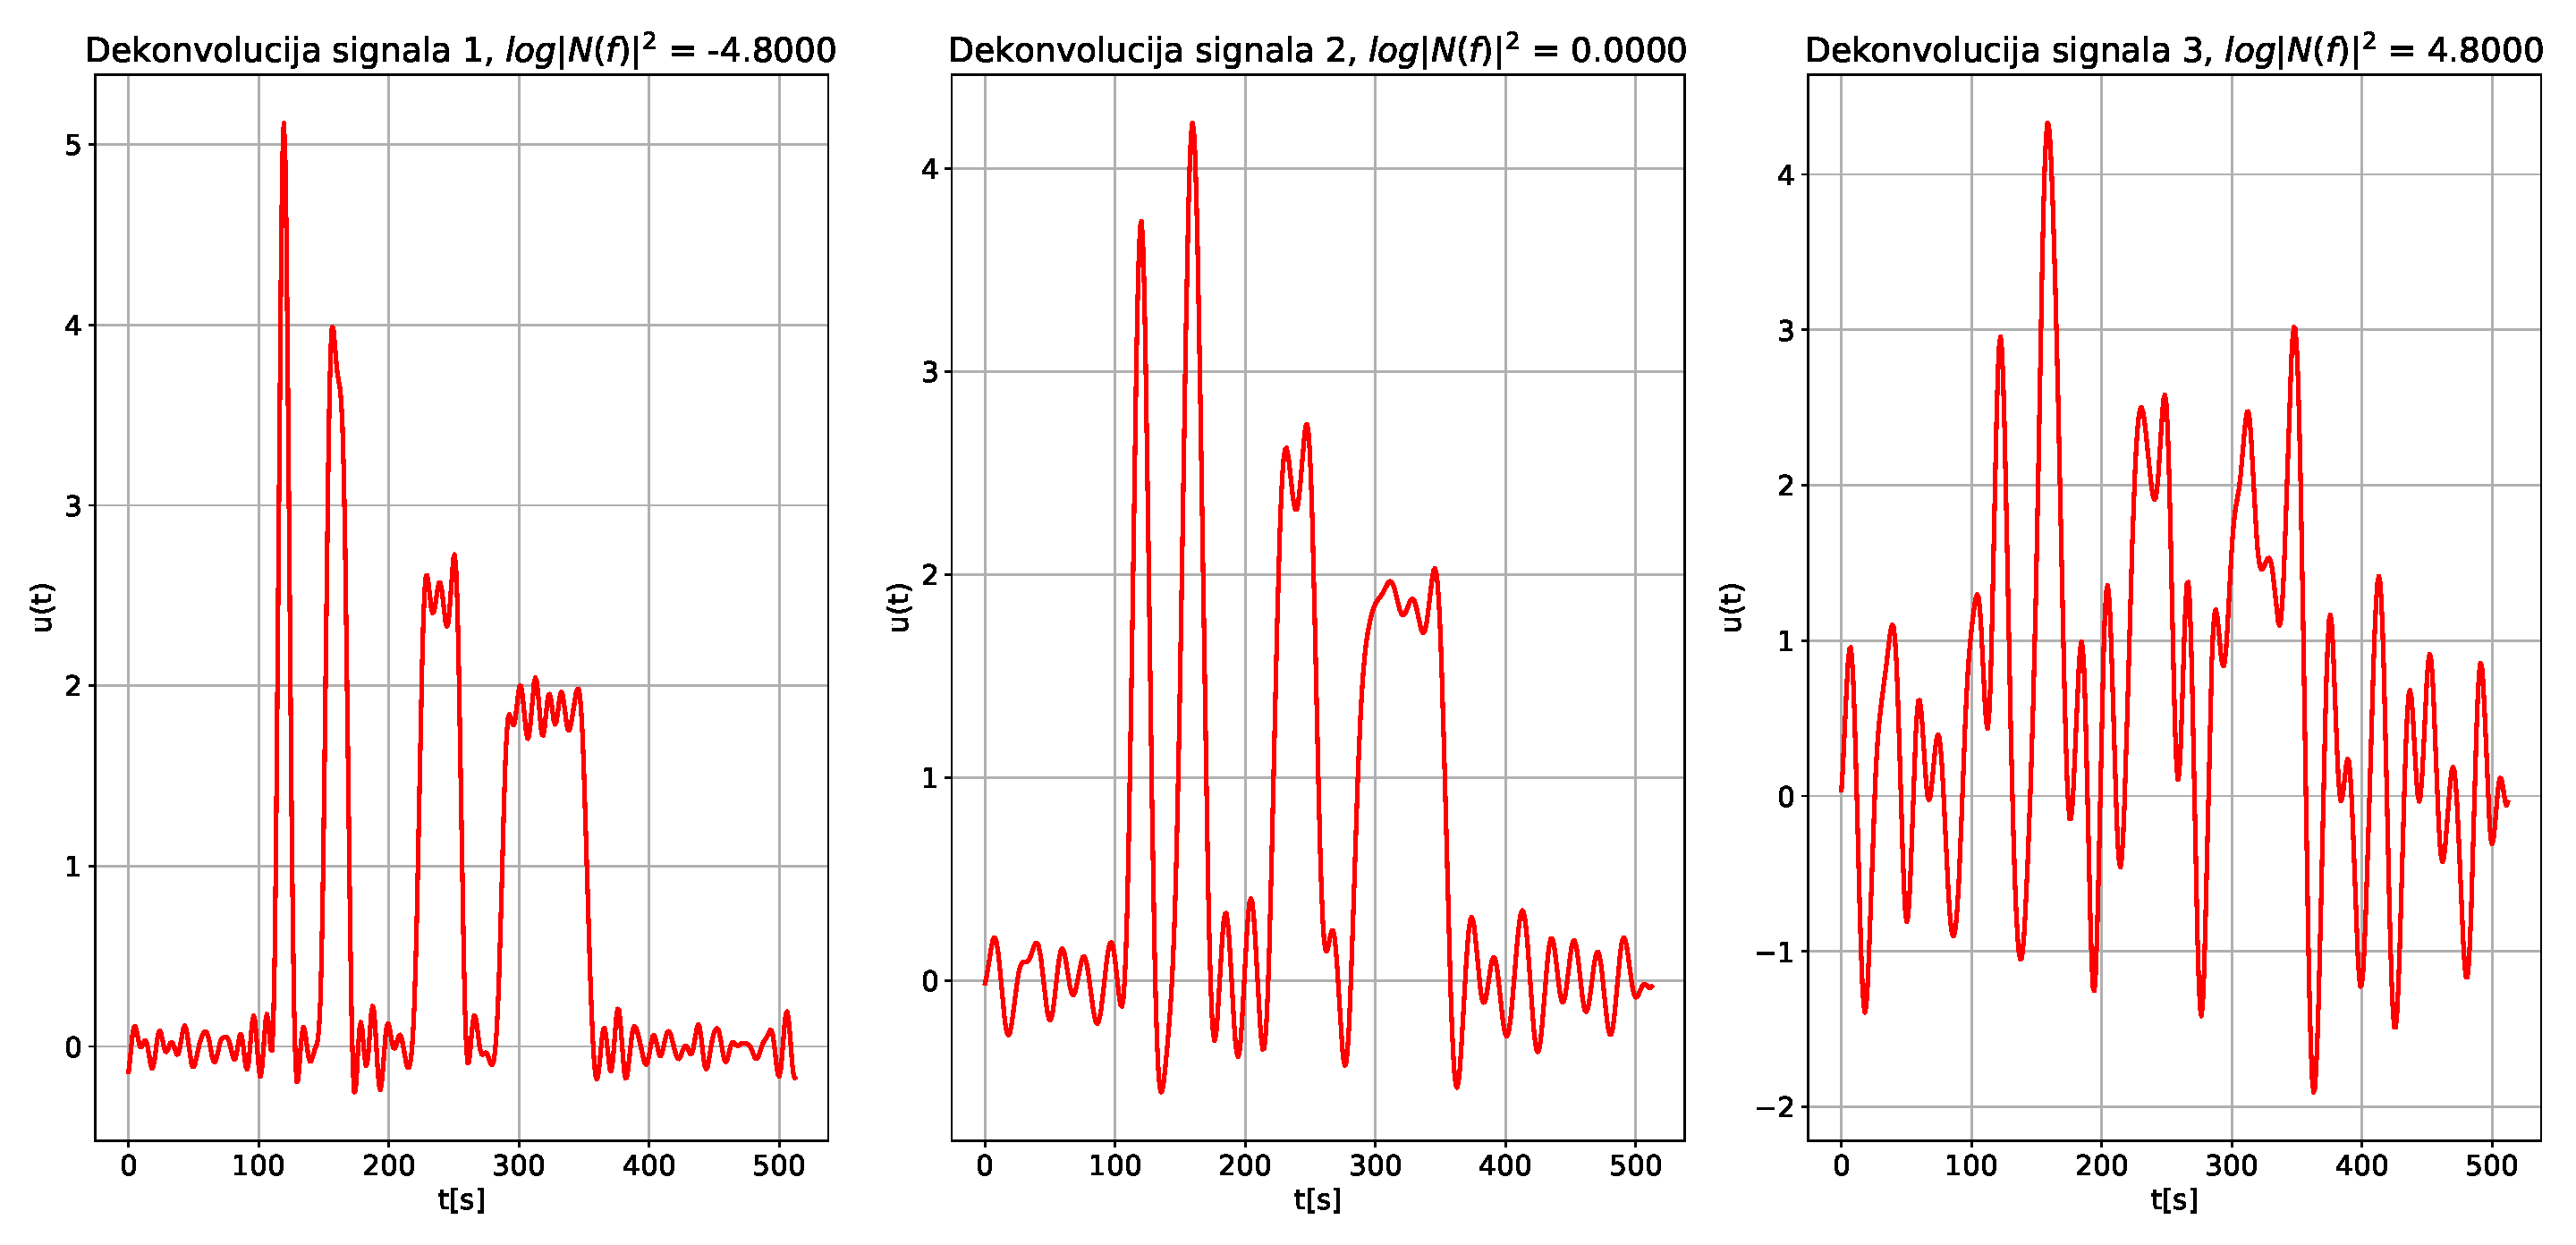
\includegraphics[width=16cm, height=6cm]{druga_drugi3dekonvolucija.pdf}
\caption{Dekonvolucija zašumljenih signalov - vidimo, da smo precej dobro ocenili vrednost signala in šuma, saj nam dekonvolucija da dobre rezultate, vendar pa vidimo, da smo za najbolj zašumljen signal ocenili premalo šuma.}  
\end{figure}
Poskusimo sedaj s več različnimi vrednosti šuma na signalu 3, ki je najbolj zašumljen
\begin{figure}[H]
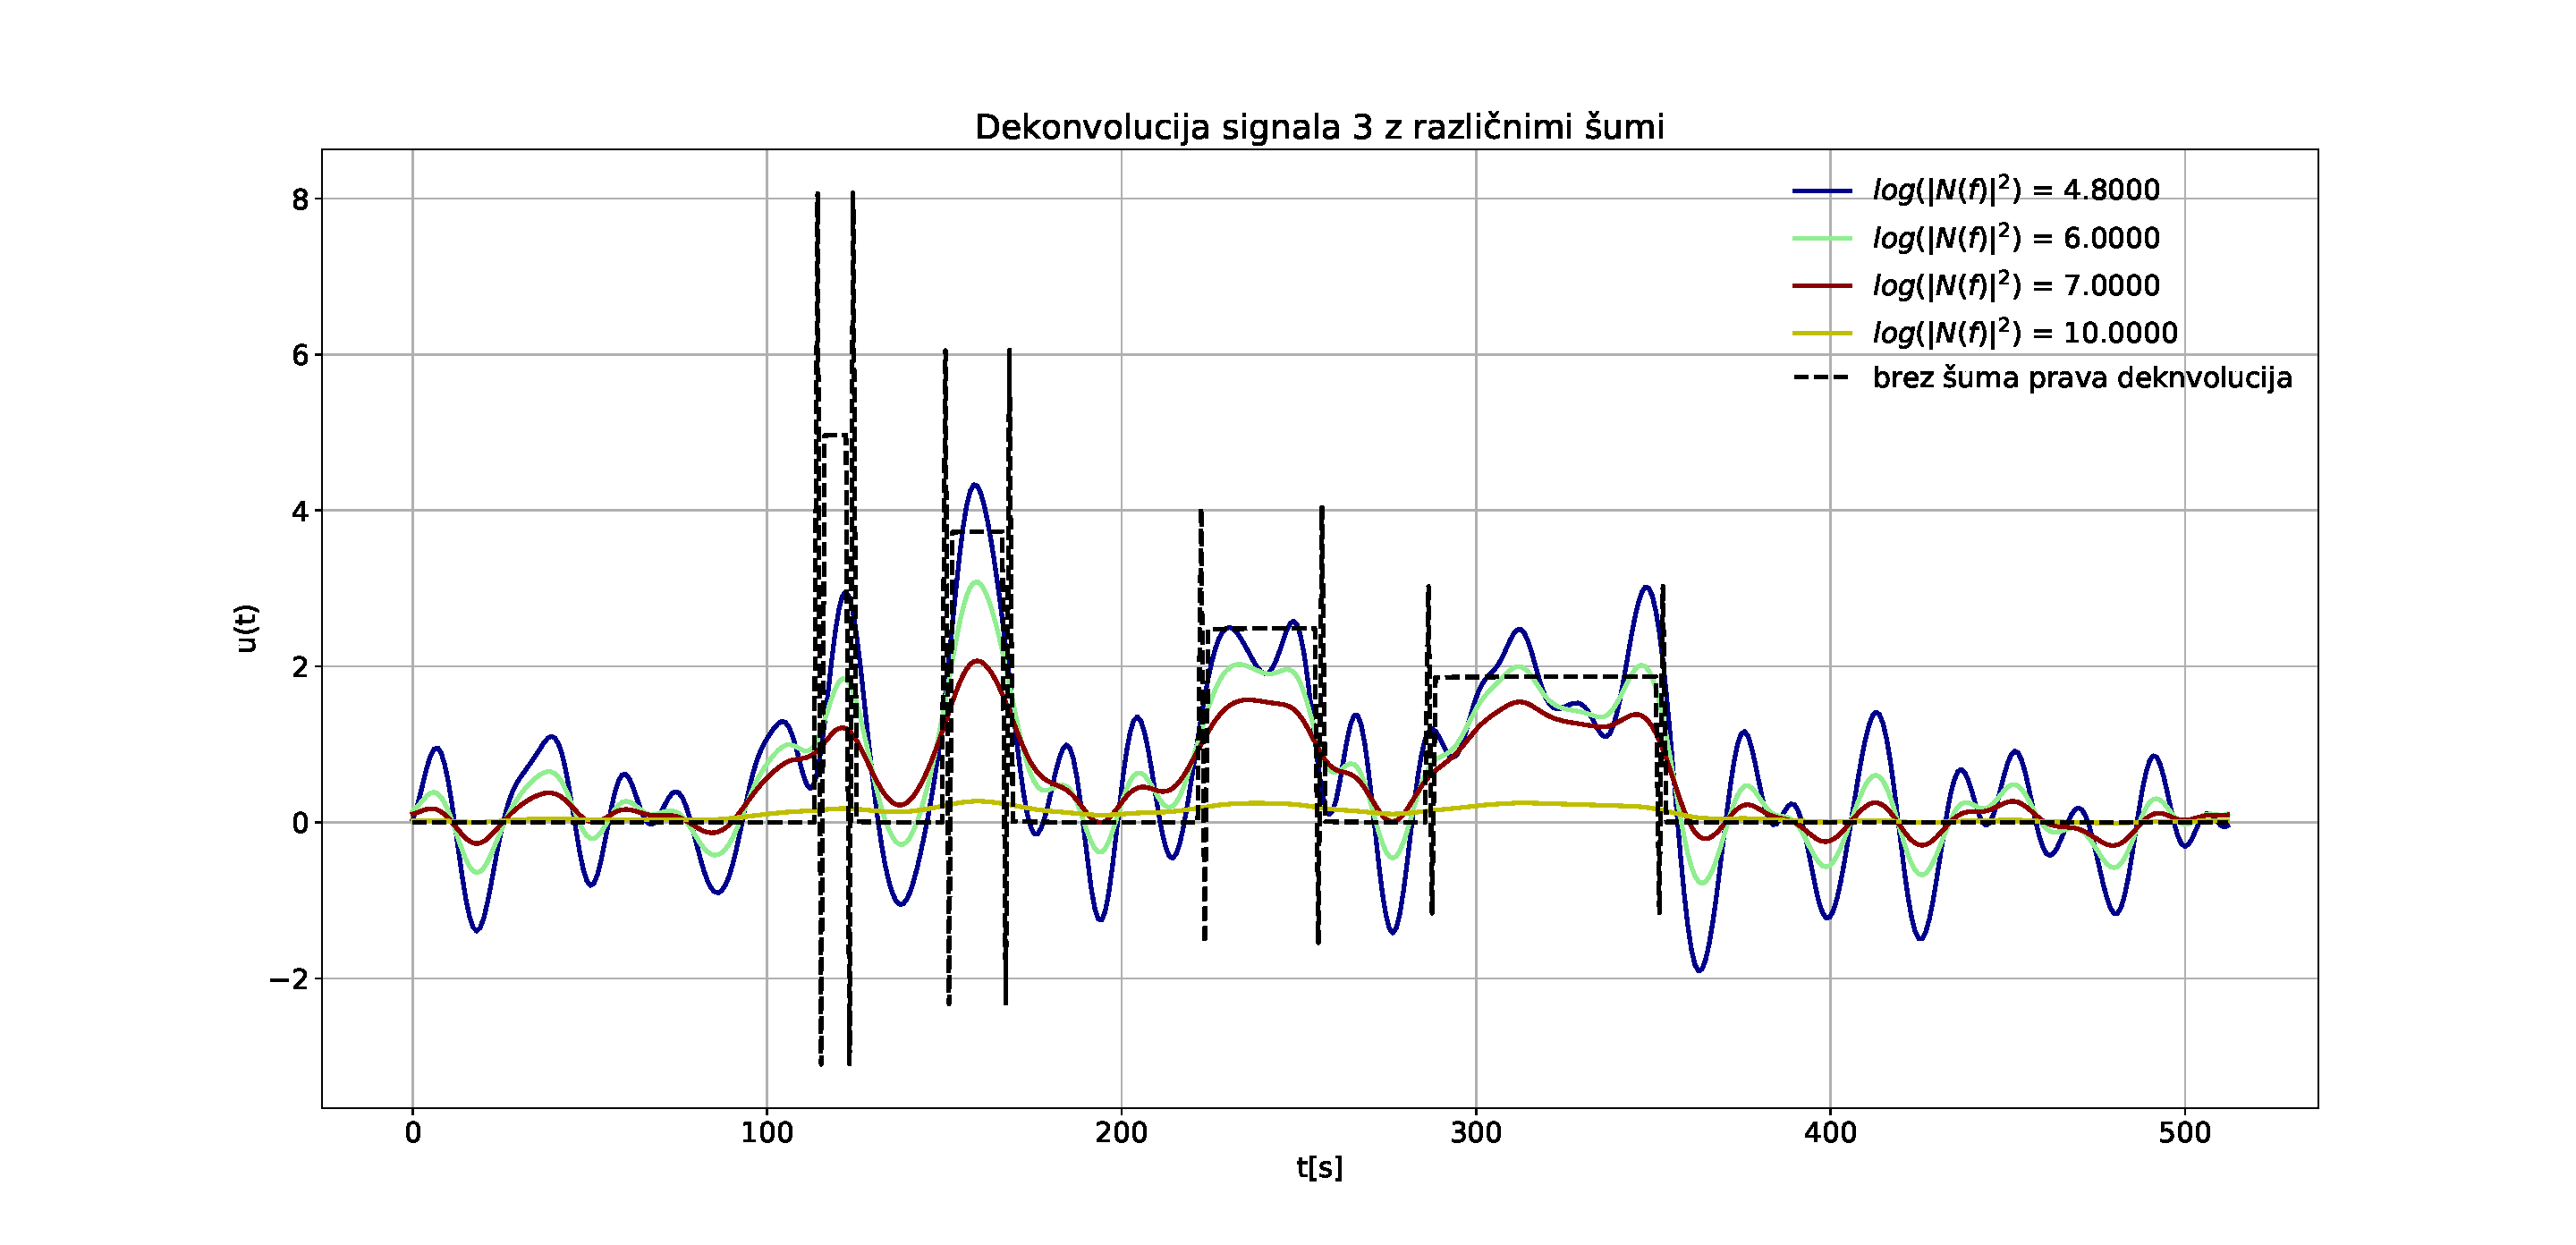
\includegraphics[width=16cm, height=8cm]{druga_prava_dekonvolucija.pdf}
\caption{Vpliv šuma na dekonvolucijski signal u(t): Vidimo, da nam prevelik šum preveč zaduši vrednosti signala (siva), med tem ko za premajhen šum (modra, 4.8) v u(t) prejmemo preveč šuma in tako signal ni razpoznaven, najboljša rešitev je tako svetlo modri šum, ki nam ojači le vrhove in zaduši stranski šum }  
\end{figure}
\subsection{Dekonvolucija slike}
Recimo da z vrstičnim tunelskim mikroskopom zajemom sliko, ki jo predstavimo s $N$ stolpci in $M$ vrsticami. To naredimo tako da odberemo vsak stolpec posebaj in si zapišemo intenziteto električnega toka/svetlobe. Ko merimo se signal žal razmaže zaradi dveh pojavov; šuma v merilnem sistemu in vpliva sosednjih izmerjenih mest na sosede. Tak vpliv vpišemo s prenosno funkcijo, npr. eksponentno
\begin{equation}
r(t) = \frac{1}{\tau} e^{-\frac{t}{\tau}}
\end{equation}
Oglejmo si primer dobljenih slik na testnem primeru Lincolna.
\begin{figure}[H]
\centering
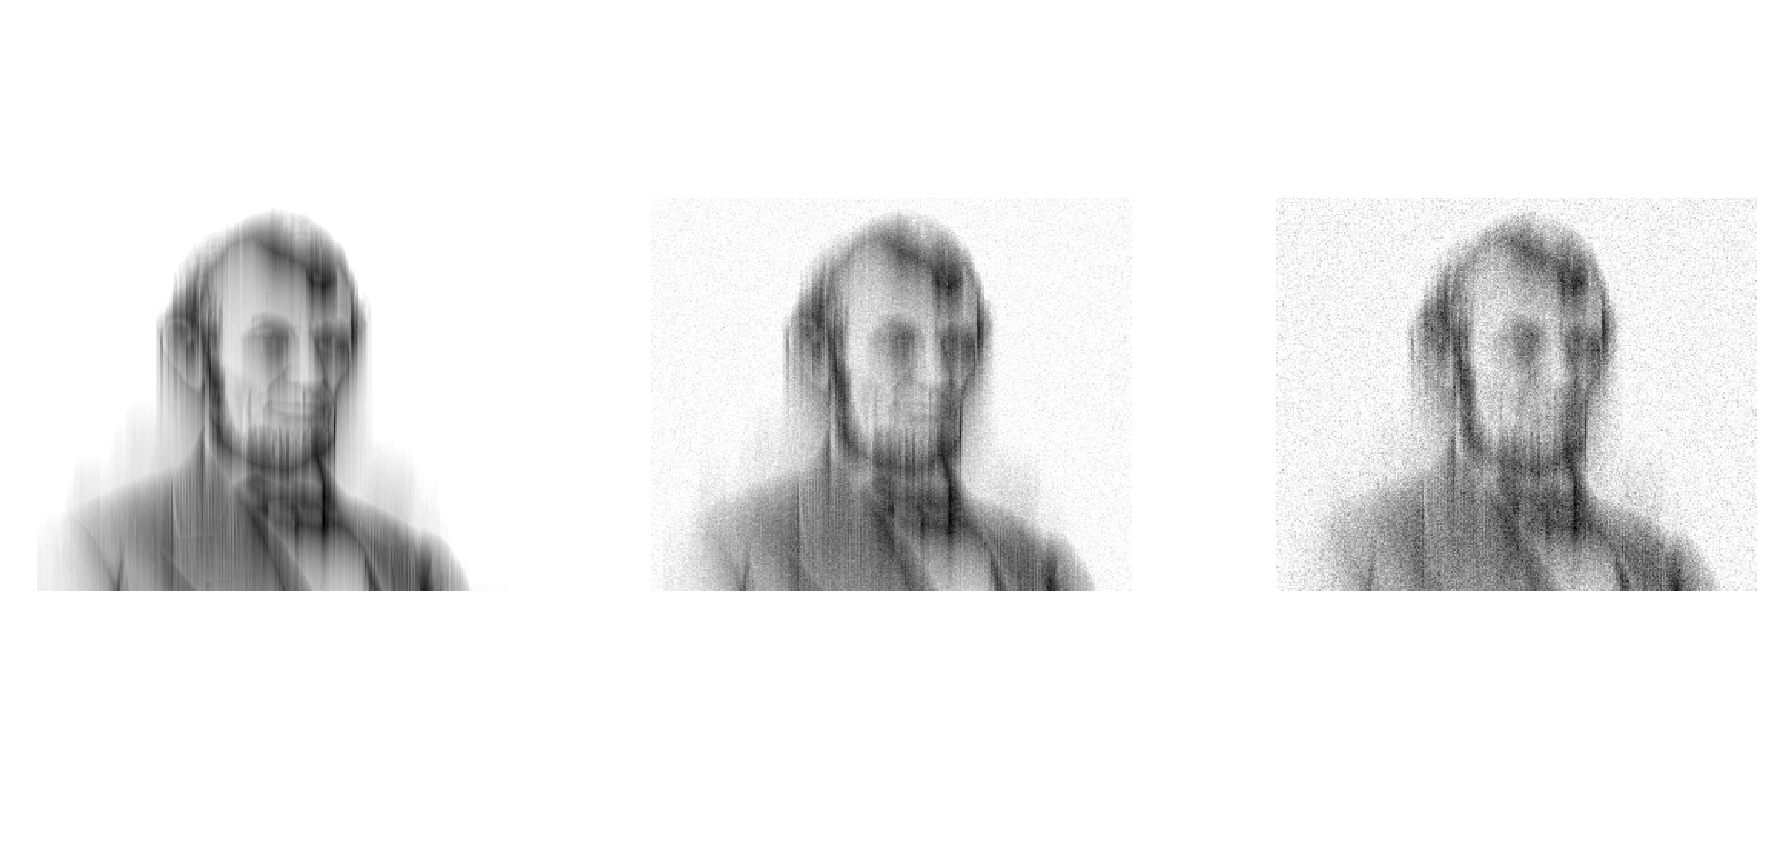
\includegraphics[width=16cm]{tretja_prvi.png}
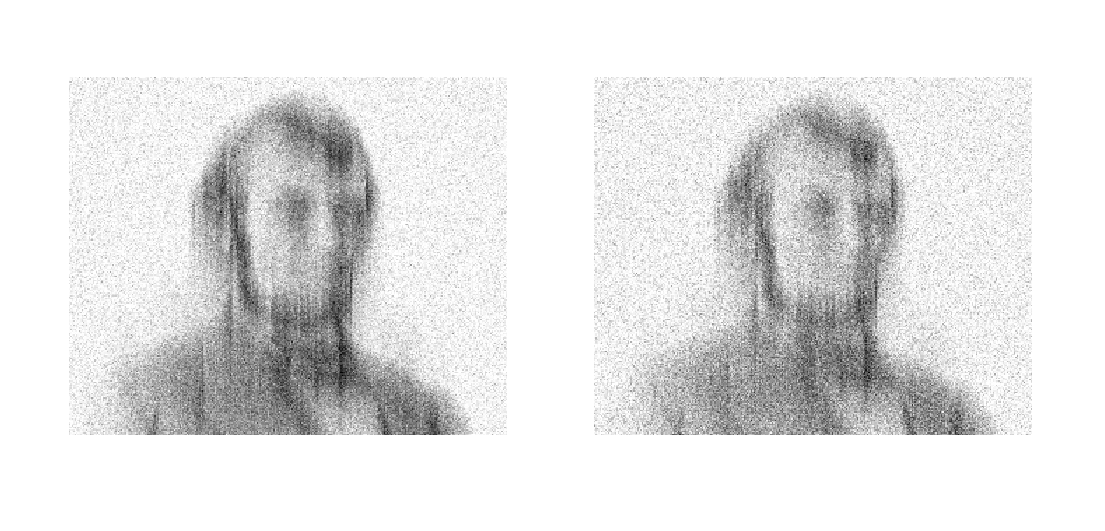
\includegraphics[width=13cm, height=5cm]{tretja_prvi1.png}
\caption{Lincolnove podobe od 1 do 5 so različno zašumljene. Prva slika je brez šuma, slike od 2-5 pa so vse zašumljene. Vse so malo izmaknjene v navpični smeri kar je vpliv konvolucije s signalom r(t).}  
\end{figure}
Vsak stolpec je tako 1D signal, ki ga moramo dekonvoluirati.
\begin{figure}[H]
\centering
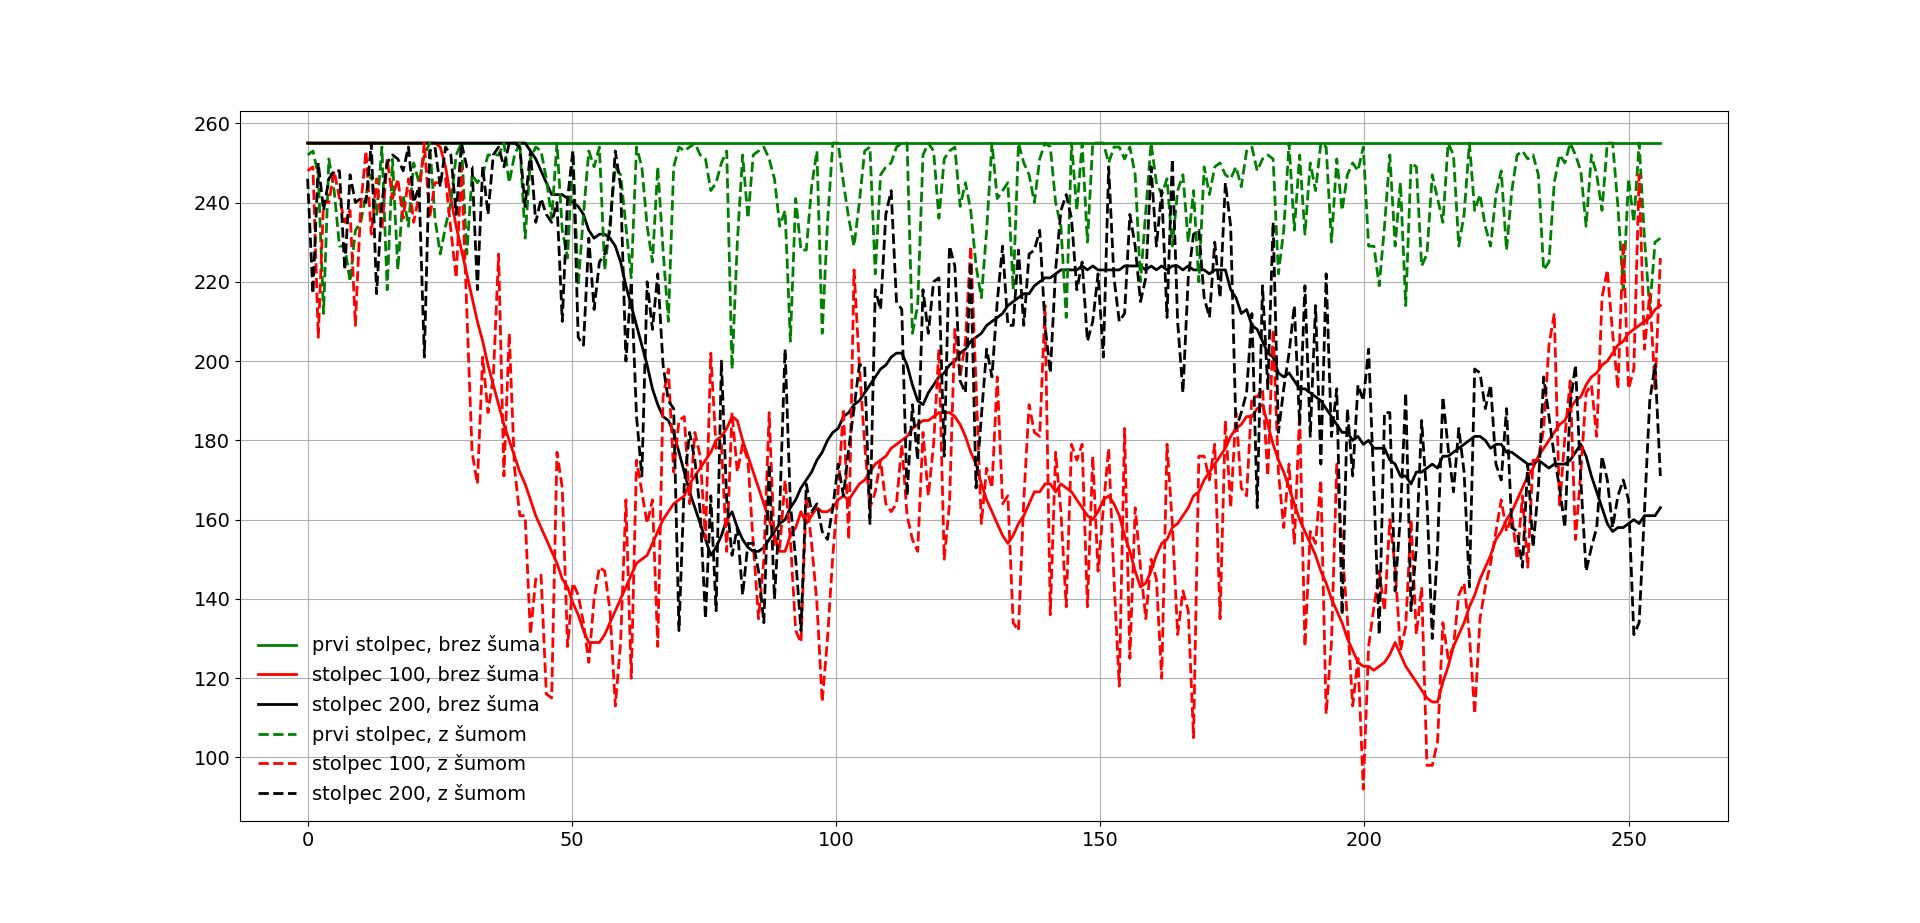
\includegraphics[width=18cm, height=6cm]{tretja_prvi2.png}
\caption{Primeri signalov. Vidimo da nam šum namesto ravne črte popači signal}  
\end{figure}
S pomočjo enačbe (12) dekonvoluiramo nezašumljeno sliko in poskusimo na zašumljenih slikah 
\begin{figure}[H]
\centering
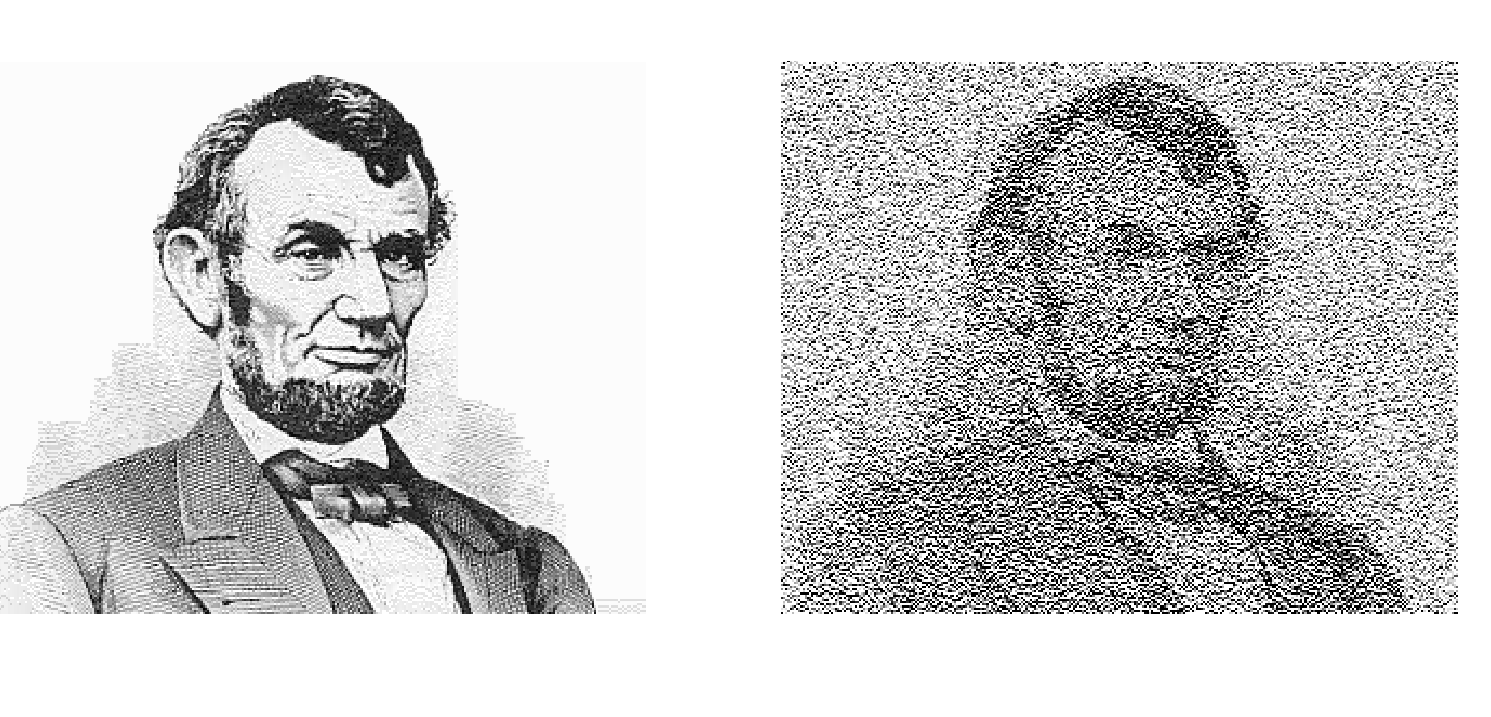
\includegraphics[width=16cm, ]{tretja_drugi.png}
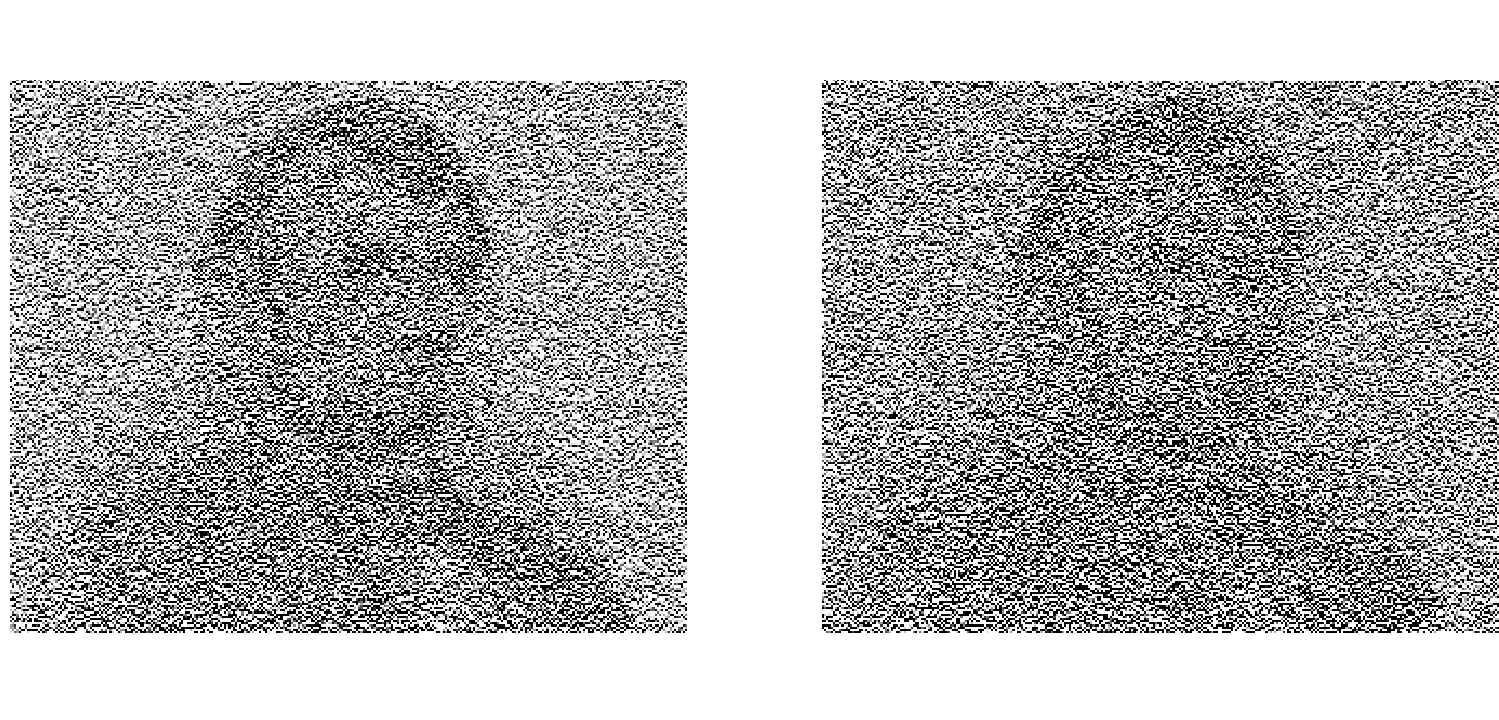
\includegraphics[width=16cm, ]{tretja_drugi2.png}
\caption{Dekonvolucijska slika Lincolna ni več popačena. Na zašumljenih slikah pa brez Wienerjevga filtra samo še povečamo šum, čeprav smo sliko načeloma dekonvoluirali.}  
\end{figure}
\subsection{Wienerjev filter}
Oceniti moramo $\Phi$. Lahko bi to storili avtomatizirano za vsak stolpec posebaj a se raje odločimo za izračun spektralne gostote povprečnega signala po stolpcih. Iz tam lahko ocenimo šume za vsako sliko in poskusimo s linearnim fitom, ki pa nam ne opiše dobro signal zato raje za $|S(f)|^2$ uporabimo kar $|C(f)|^2$, ki pa mu porežemo visoke frekvence, kjer je spektralna moč le še konstantna.
\begin{figure}[H]

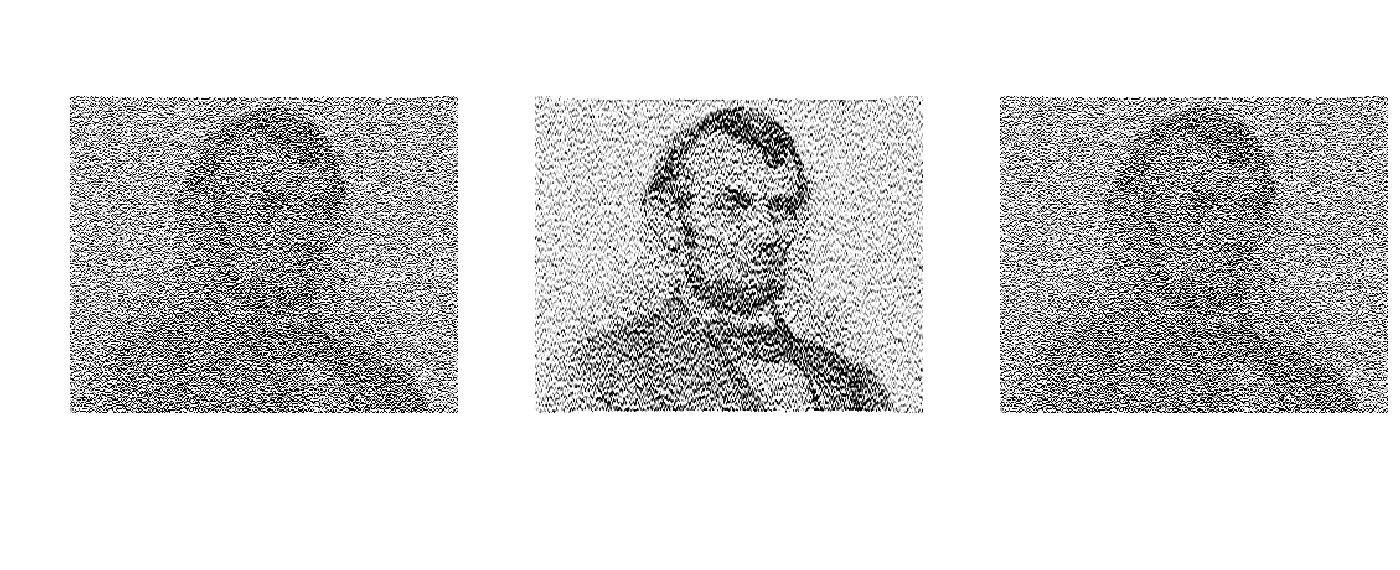
\includegraphics[width=16cm, ]{tretja_drugi5.png}
\caption{Linearni poskus se izjalovi.}  
\end{figure}
Če preprosto odrežemo del signala in ga uporabimo v Wienrjev filter dobimo že dosti boljše rezultate.
\begin{figure}[H]
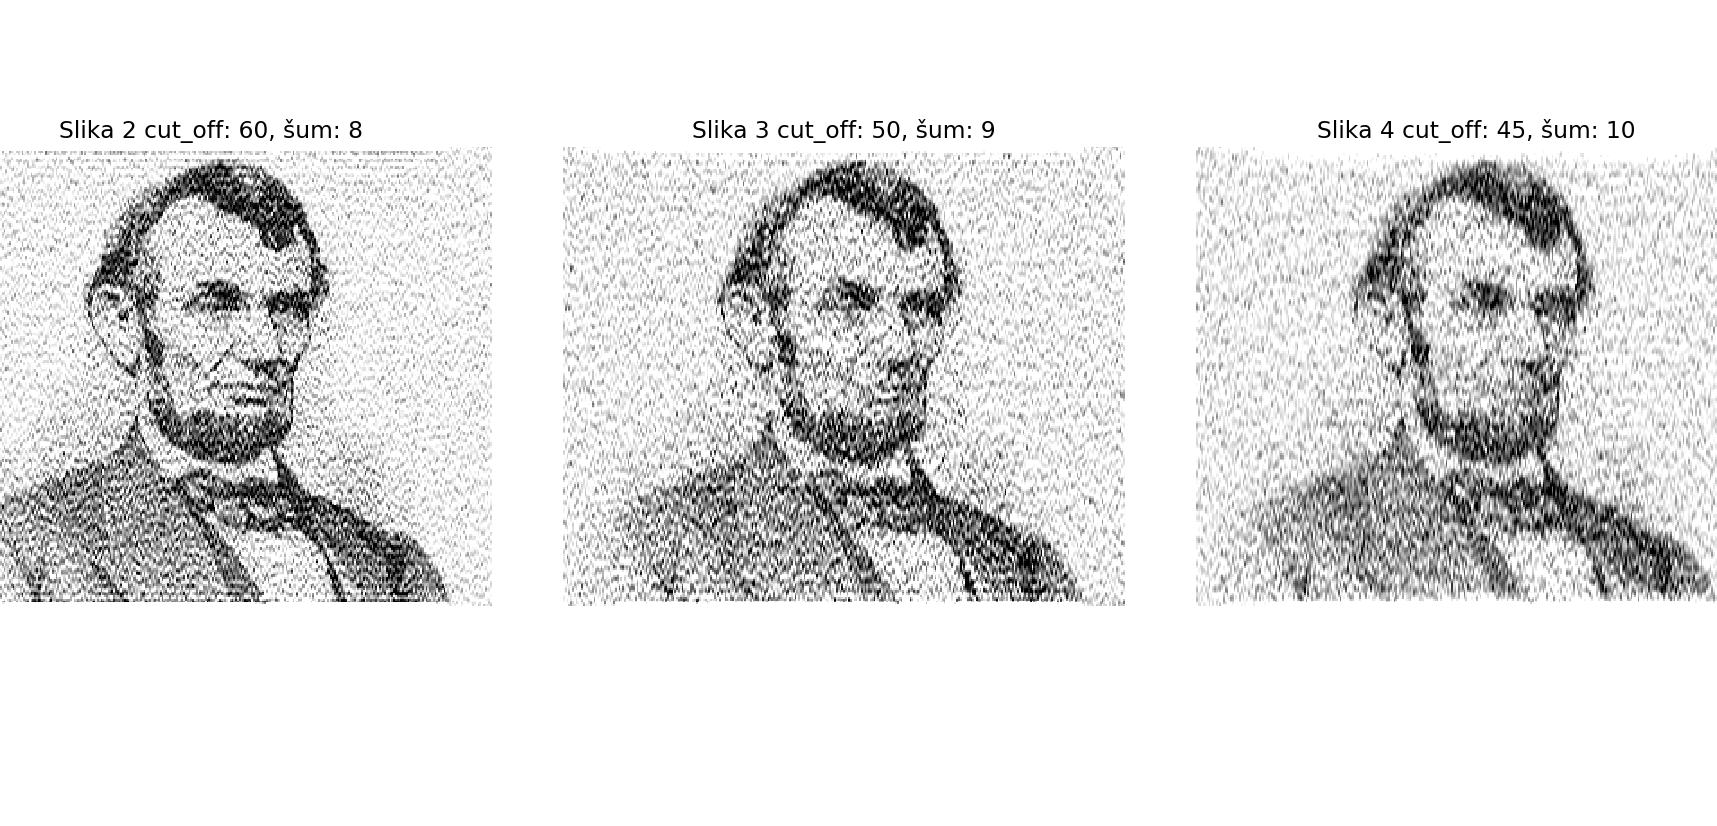
\includegraphics[width=16cm, ]{tretja_tretji1.png}

\caption{Prikaz slik po zašumljenosti od leve proti desni. Iz grafa spektralnih moči vidimo, da je cut off za bolj zašumljene slike večji. Čeprav so slike dekonvoluirane pa imajo naslednje probleme. Niso ostre, in ostajajo zašumljene. Poskusimo se znebiti šuma tako da na graf fitamo eksponent in nato odrežemo signal, stem pa spektralna moč postane bolj gladka.}  
\end{figure}
Čeprav so slike dekonvoluirane kljub šumu, pa imajo naslednje probleme. Niso ostre, in ostajajo zašumljene. Poskusimo se znebiti šuma tako da na graf fitamo eksponent in nato odrežemo signal, stem pa spektralna moč postane bolj gladka. Najprej si poglejmo vpliv velikosti cut off frekvence na sliki 4.

Poskusimo s eksponetnim fitom, da bi zmnajšali šum 
\begin{figure}[H]

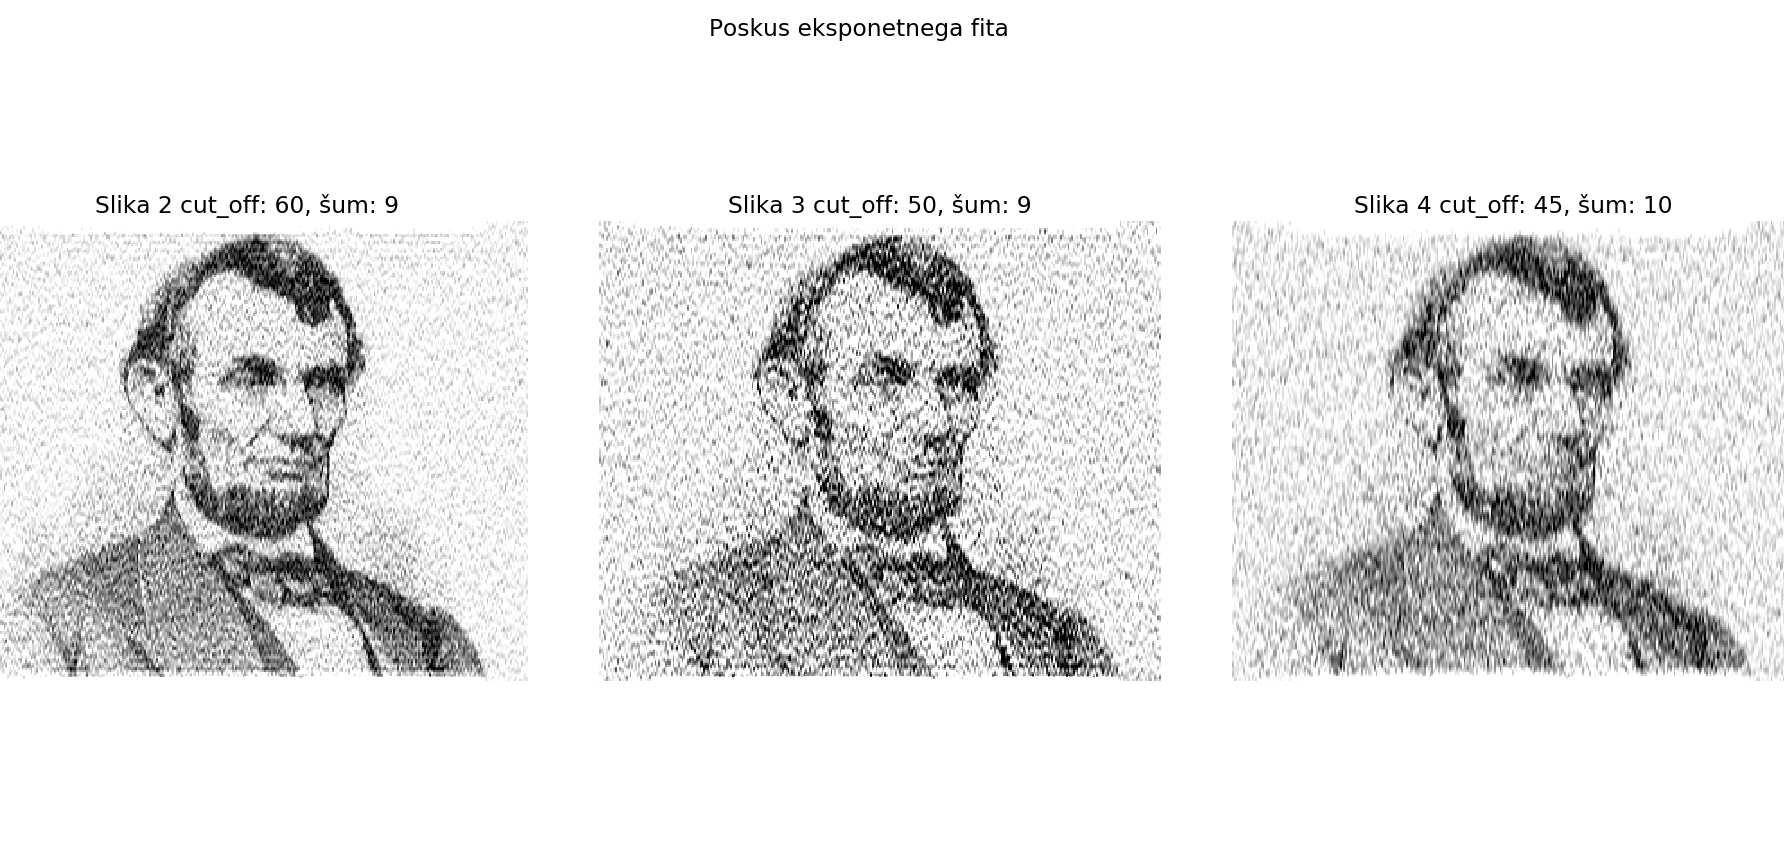
\includegraphics[width=16cm, ]{tretja_tretji4.png}
\caption{Eksponetni fit s istimi parametri kot na sliki 16. Vidimo, da se tako znebimo zašumljenosti v primerjavi s sliko 16. }  
\end{figure}

\begin{figure}[H]

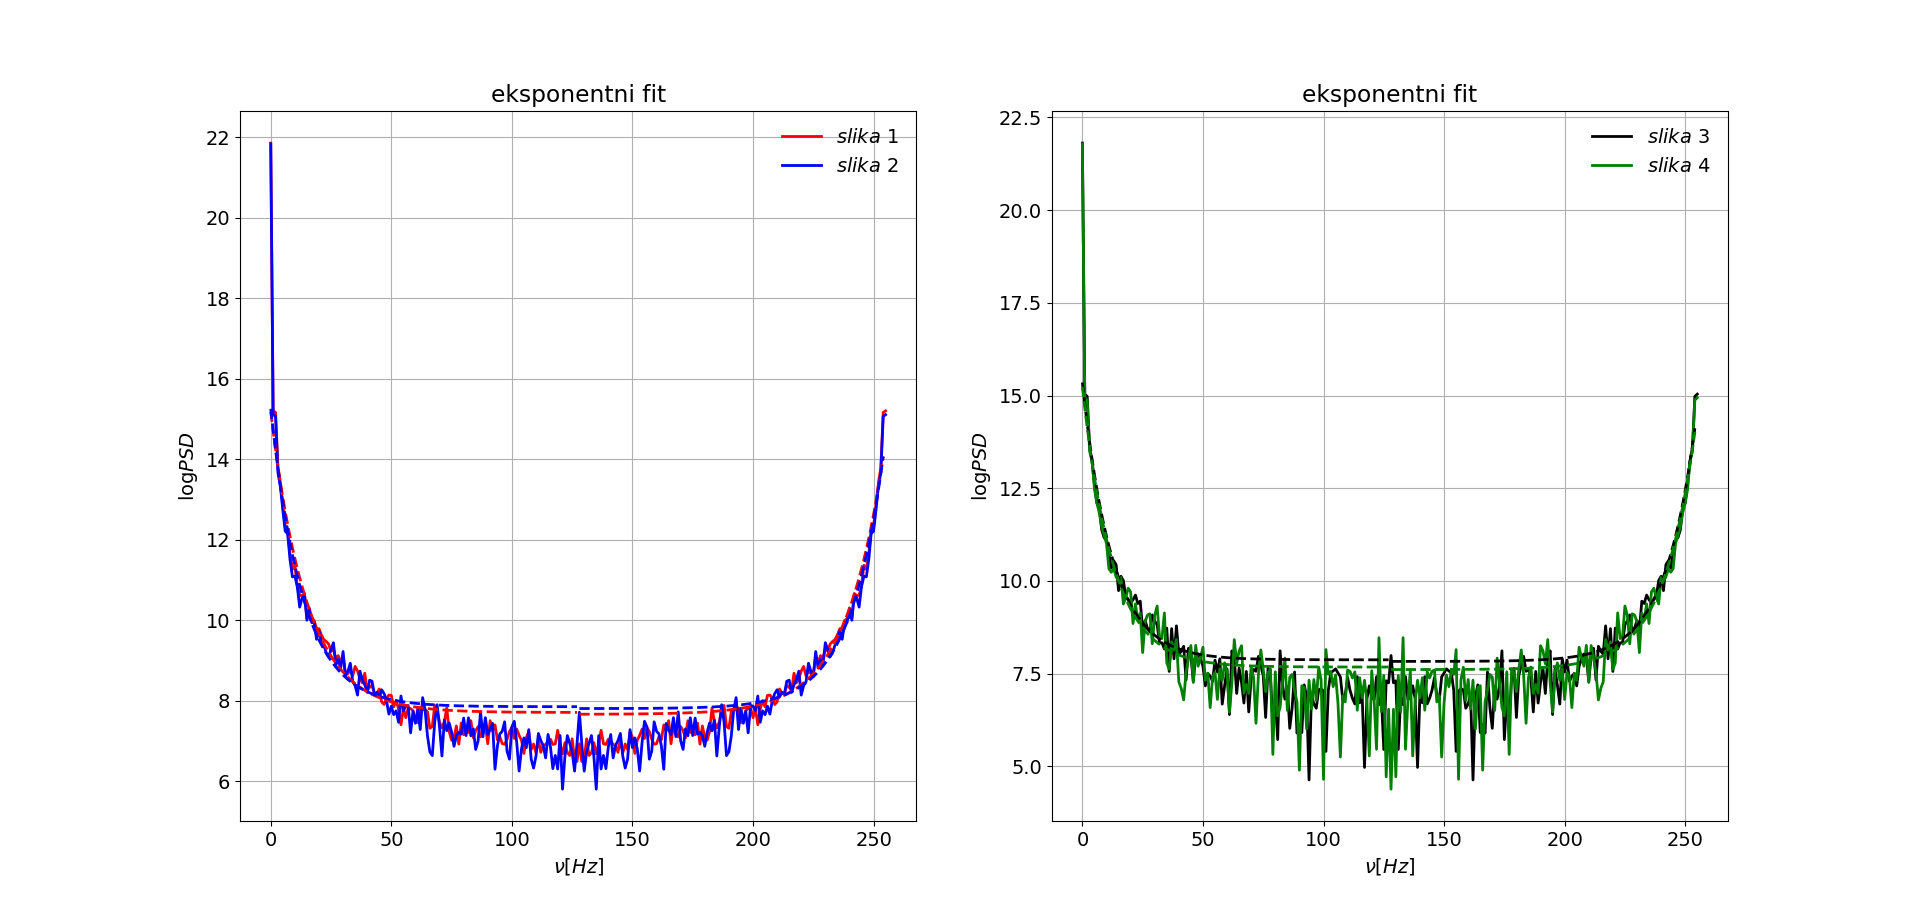
\includegraphics[width=18cm, height=6cm]{tretja_tretji3.png}

\caption{Eksponetni fit. }  
\end{figure}
\subsection{Vpliv cut off na sliko}
\begin{figure}[H]
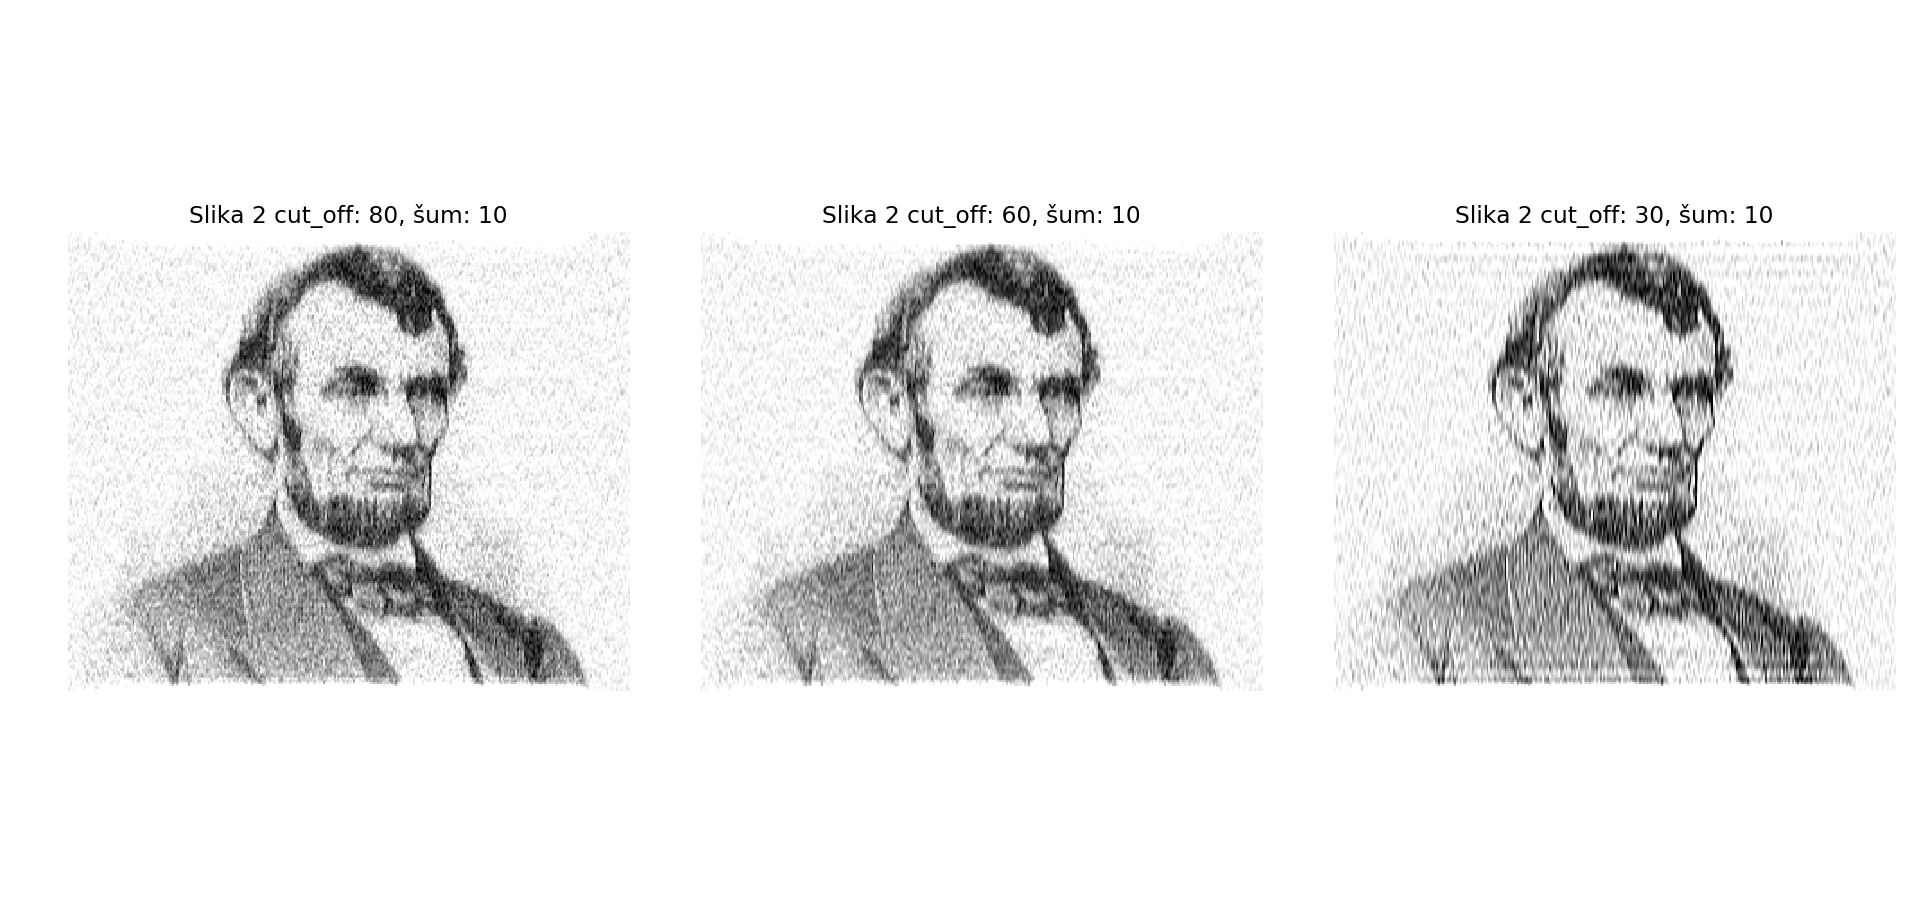
\includegraphics[width=16cm, ]{tretja_tretji2.png}

\caption{Cut off {60,45,35 Hz} na sliki 2 (rahlo zašumljena ) nam poreže vedno višje frekvence, zato je slika manj ostra od leve proti desni, }  
\end{figure}
Za izboljšanje slike bi morali avtomatizirati iskanje Winerjevega filtra na vsakem signalu in nato dekonovoluirati vsak stolpec s ustreznim $\Phi$. S slikami ki smo jih dobili iz povprečenja smo vseeno zadovoljni saj pri dovolj močnem šumu težko zares očistimo sliko.

\section{Zaključek}
Naučili smo se kako dekonvoluirati signale in vpliv okenskih funkcij za izboljšavo fourierove transformacije. Pogledali smo si tudi praktičen primer dekonvolucije in filtriranja slik.


\end{document}